\documentclass{tufte-handout}

%\geometry{showframe}% for debugging purposes -- displays the margins

\usepackage{amsmath}


% Set up the images/graphics package
\usepackage{graphicx}
\setkeys{Gin}{width=\linewidth,totalheight=\textheight,keepaspectratio}
\graphicspath{{graphics/}}


% The following package makes prettier tables.  We're all about the bling!
\usepackage{booktabs}

% The units package provides nice, non-stacked fractions and better spacing
% for units.
\usepackage{units}

% The fancyvrb package lets us customize the formatting of verbatim
% environments.  We use a slightly smaller font.
\usepackage{fancyvrb}
\fvset{fontsize=\normalsize}

% Small sections of multiple columns
\usepackage{multicol}

% Provides paragraphs of dummy text
\usepackage{lipsum}

% Provides annotated music scores
\usepackage{musicography}

% Fancy header
\usepackage{fancyhdr}

\usepackage{array, boldline, makecell, booktabs}

\newcommand{\bmp}[1]{\begin{minipage}{#1}}
\newcommand{\emp}{\end{minipage}}
\newcommand{\tw}{\textwidth}

% These commands are used to pretty-print LaTeX commands
\newcommand{\doccmd}[1]{\texttt{\textbackslash#1}}% command name -- adds backslash automatically
\newcommand{\docopt}[1]{\ensuremath{\langle}\textrm{\textit{#1}}\ensuremath{\rangle}}% optional command argument
\newcommand{\docarg}[1]{\textrm{\textit{#1}}}% (required) command argument
\newenvironment{docspec}{\begin{quote}\noindent}{\end{quote}}% command specification environment
\newcommand{\docenv}[1]{\textsf{#1}}% environment name
\newcommand{\docpkg}[1]{\texttt{#1}}% package name
\newcommand{\doccls}[1]{\texttt{#1}}% document class name
\newcommand{\docclsopt}[1]{\texttt{#1}}% document class option name


%%% Additions to template by DSL
\usepackage{hyperref} % provides \url{}
% remove separation between list items http://tex.stackexchange.com/a/10689/1783
\usepackage{enumitem}
\setlist{nosep}

%%-- another way
\usepackage{tikzpagenodes}
\newcommand{\mylogo}[1]{%
\tikz[remember picture,overlay] {%
  \node[inner sep=0pt,anchor=east] at ([yshift=+1.0cm, xshift=+7.0cm]current page text area.north east){#1};}
  }

\usepackage{mathrsfs}
\usepackage{tcolorbox}
\tcbuselibrary{theorems}
\usepackage{xcolor}
\usepackage{epsdice}
\usepackage{pgfplots}

\usepackage{graphicx,xspace,color,cancel}
\usepackage{tikz}
\usetikzlibrary{arrows,shapes,backgrounds,through,shadows}
\usetikzlibrary{decorations.pathmorphing}
\usetikzlibrary{calc}

\newcommand{\boxit}[4]
{
\path #2+(-#4,-#4) node(bottomleft){};
\path #3+(#4,#4) node(upperright){};
\draw[rounded corners,black!80] (bottomleft) rectangle (upperright);
%\path (#2-|#3) node(bottomright){};
\path (bottomleft-|upperright) node(bottomright){};
\path (bottomright) node[above left]{#1};
}

\tikzstyle{cont}=[circle, draw,% a shading that is white at the top...
thick,minimum size=6mm,line width=1pt,>=stealth]  % continuous  node
\tikzstyle{dgraph}=[->, line width=1.5pt]

\tikzstyle{contblk}=[circle, draw=black,top color=black,bottom color=black,% a shading that is white at the top...
thick,minimum size=1mm,line width=1pt,>=stealth]  % continuous  node
\tikzstyle{dgraph}=[->, line width=1.5pt]



\newtcbtheorem[number within=]{mydef}{Definition}%
{colback=DarkOrchid!5,colframe=DarkOrchid!90!black,fonttitle=\bfseries}{th}

\newtcbtheorem[number within=]{mydef2}{Definition$^*$}%
{colback=Rhodamine!5,colframe=Rhodamine!90!black,fonttitle=\bfseries}{th}


\newtcbtheorem[number within=]{mybox}{Box}%
{colback=Aquamarine!5,colframe=Aquamarine!90!black,fonttitle=\bfseries}{th}

\newtcbtheorem[number within=]{mybox2}{Box$^*$}%
{colback=gray!5,colframe=gray!90!black,fonttitle=\bfseries}{th}

\newtcbtheorem[number within=]{mythe}{Theorem}%
{colback=DarkOrchid!5,colframe=DarkOrchid!90!black,fonttitle=\bfseries}{th}



% \bigcupdot
\makeatletter
\def\moverlay{\mathpalette\mov@rlay}
\def\mov@rlay#1#2{\leavevmode\vtop{%
   \baselineskip\z@skip \lineskiplimit-\maxdimen
   \ialign{\hfil$\m@th#1##$\hfil\cr#2\crcr}}}
\newcommand{\charfusion}[3][\mathord]{
    #1{\ifx#1\mathop\vphantom{#2}\fi
        \mathpalette\mov@rlay{#2\cr#3}
      }
    \ifx#1\mathop\expandafter\displaylimits\fi}
\makeatother
\newcommand{\cupdot}{\charfusion[\mathbin]{\cup}{\cdot}}
\newcommand{\bigcupdot}{\charfusion[\mathop]{\bigcup}{\boldsymbol{\cdot}}}

%\rhead{\includegraphics[width=1cm]{fig/T1.png}}
\def\ci{\perp\!\!\!\perp}

\title{Probability Theory  }
\author{Salvador Ruiz Correa}
\date{August 18, 2025}  % if the \date{} command is left out, the current date will be used
\begin{document}

\maketitle% this prints the handout title, author, and date
\mylogo{\includegraphics[height=15mm]{fig/T2.png}}

\begin{abstract}


This section introduces the foundational concepts of probability distributions and their continuous and discrete representations. We begin by defining probability distributions as mathematical functions that assign likelihoods to outcomes within a sample space. For discrete random variables, this takes the form of a probability mass function (PMF), while for continuous random variables, it is described by a probability density function (PDF). We explore the properties and interpretations of these functions, emphasizing their roles in quantifying uncertainty and modeling real-world phenomena.
The discussion then extends to cumulative distribution functions (CDFs), which capture the probability that a random variable takes a value less than or equal to a given threshold. Both discrete and continuous cases are treated, highlighting the differences in their behavior and analytical structure. Key relationships between PMFs, PDFs, and their respective CDFs are established, and graphical illustrations are used to reinforce intuition.
By the end of this section, readers will have a clear understanding of how probability distributions and densities encapsulate randomness, and how cumulative functions provide a powerful tool for analyzing probabilistic events over intervals.

\end{abstract}
\marginnote[-5cm]{
\textsc{Agenda:}
\begin{description}
\item{1} Probability distribution function.
\item{2} Probability density function.
\item{3} Cumulative dstribution function.
\item{4} Cummulative density function
\end{description}
}


\begin{marginfigure}
\centering
\includegraphics{fig/disc.png}

\caption{Probability distribution  $P(K=k) $ in  Table 1.
}
\end{marginfigure}

\subsection{Examples of Probability Distributions for Discrete Random Variables}
\begin{itemize}
\item Let $(\Omega,\mathscr F)$ describe throwing two fair dice, i.e. $\Omega:= \{(i,k): \mathsf 1\leq i,k\leq \mathsf 6\}$, $\mathscr F = \mathscr P (\Omega)$, and $P(\{i,j\}) = \mathsf{\frac{1}{36}}$. The total number of points thrown $X: \Omega \rightarrow \mathsf{\{2,3,\dots, 12\}}$, $X((i,j))=i+j$ is a measurable map (Table 1 and Figure 21).
\begin{table}[tbh]
\caption{The distribution of the random variable $X$.}
\renewcommand{\arraystretch}{1.5}
\begin{tabular}{cccccccccccc} 
\hlineB{1.5}\hline\hline
$k$ & $\mathsf 2$ & $\mathsf 3$ & $\mathsf 4$ & $\mathsf 5$ & $\mathsf 6$ & $\mathsf 7$ & $\mathsf 8$ & $\mathsf 9$ & $\mathsf 10$ & $\mathsf 11$ & $\mathsf 12$ \\\hline
$P(X= k)$ & $\mathsf{\frac{1}{36}}$  & $\mathsf{\frac{1}{18}}$ & $\mathsf{\frac{1}{12}}$ & $\mathsf{\frac{1}{9}}$ & $\mathsf{\frac{5}{36}}$ & $\mathsf{\frac{1}{6}}$ & $\mathsf{\frac{5}{36}}$ & $\mathsf{\frac{1}{9}}$ & $\mathsf{\frac{1}{12}}$ & $\mathsf{\frac{1}{18}}$ & $\mathsf{\frac{1}{36}}$ \\
\hlineB{1.5}
\end{tabular}
\end{table}
\vspace{.2cm}
\item The \textit{ Bernoulli random} variable $X\in\{0,1\}$ with parameter $\mathsf p$,  $0<\mathsf p\leq 1$ has the following probability distribution:
\begin{equation*}
P(X=x\mid \mathsf p) := \mathsf{Bernoulli}(X=x\mid \mathsf p) =  \mathsf p^x(1-\mathsf p)^{1-x} .
\end{equation*}
Hint: $P(X=1\mid \mathsf p) = \mathsf p$.

\begin{marginfigure}
\centering
\includegraphics{fig/binomial.png}

\caption{Binomial probability distribution function for $N=20$ and $p=0.5$.
}
\end{marginfigure}

\item The \textit{Binomial distribution} with parameters $\mathsf N$ and $\mathsf p$ is the discrete probability distribution of the number $K$ of successes in a sequence of $\mathsf N$ independent Bernoulli trials (with parameter $\mathsf p$). The probability distribution is

\begin{equation*}
P(K=k\mid {\mathsf N},\mathsf p) := \mathsf{Binomial}(K=k\mid \mathsf p,\mathsf N)  = {{\mathsf N}\choose k} \mathsf p^k\mathsf{(1- p)}^{{N}-k} \,\,\,\, 
\end{equation*}
$ \text{for } \,\,\,\, k = 0,1,2,\dots$ where $${{\mathsf N}\choose k} = \frac{{\mathsf N}!}{({\mathsf N}-k)!k!}$$ is the number of ways of choosing $K=k$ objects out of a total of $ \mathsf N$ identical objects.
\end{itemize}

\begin{marginfigure}
\centering
\includegraphics{fig/binomial2.png}

\caption{Binomial probability distribution function for $N=20$ and $p=0.6$.
}
\end{marginfigure}


\section{Continuous Random Variables }

A random variable $X$ is a continuous random variable if there exists a non-negative function $f_X(\cdot)$ such that:
\begin{align*}
P(X\leq \omega) = \int_{-\infty}^\omega f_X(\alpha)d\alpha
\end{align*}
for any $\omega\in \mathbb R$. The function $f_X$ is called the probability density function of $X$. To simplify notation in practice we use $p(x) = f(x) = f_X(x)$. We remark on the abuse of notation.

\begin{marginfigure}
\centering
\includegraphics{fig/beta3.png}

\caption{Beta probability density function. $\alpha=2$, $\beta=5$ (dark green), $\alpha=2$, $\beta=2$ (lime green).
}
\end{marginfigure}
\section{Examples  of Continuous Random Variables } 
\begin{itemize}
\item A  random variable $M\in[0,1]$ has a Beta distribution of variable with parameters $\alpha$ and $\beta$ if the density function has the form
  \begin{equation*}
  f_M(m\mid \alpha,\beta) := \mathsf{Beta}(m \mid \alpha,\beta)  = \frac{\Gamma(\alpha+\beta)}{\Gamma(\alpha)\Gamma(\beta)} m^{\alpha-1}(1-m)^{\beta-1},
  \end{equation*}
  where $\Gamma(x)$ is the Gamma function  $\Gamma(x)=\int_0^{x} u^{x-1} e^{-u}  du$.
  
\begin{marginfigure}
\centering
\includegraphics{fig/gauss2.png}

\caption{Gaussian probability density function. $\mu=0$, $\sigma^2=3$ (dark green), $\mu=2$, $\sigma^2=2$ (lime green).
}
\end{marginfigure}

 \item A  random variable $X\in \mathbb R$ has a Gaussian or Normal distribution of variable with parameters $\mu$ and $\sigma^2$ if the density function has the form
   \begin{equation*}
  f_X(x\mid \mu,\sigma^2) := \mathcal{N}(x \mid\mu,\sigma^2)  = \frac{1}{\sqrt{2\pi\sigma^2}} \exp\{-\frac{1}{2\sigma^2} (x-\mu)^2\},
  \end{equation*}
\end{itemize}



\section{ Cummulative Distribution Function}
For a random variable $X$, its cumulative distribution function (CDF) is defined as:
\begin{align*}
F_X(  x) := P(X \leq   x), \,\,\,\,   -\infty \leq  x \leq \infty
\end{align*}
Note that $P(X \leq  x) = P\circ X^{-1}((-\infty, x])$, and:
\begin{marginfigure}
\centering
\includegraphics{fig/Fx.png}

\caption{Cumulative distribution of the random variable $X$ in Table 1.
}
\end{marginfigure}
\begin{itemize}
\item $F_X(  x)$ is non-decreasing and right-continuous.
\item $\lim_{ x\rightarrow \infty} F_X( x)= 1$ and 
\item $\lim_{  x\rightarrow -\infty} F_X( x)= 0$
\end{itemize}

Conversely, if a given function $F_X$ satisfies the above properties, then it is a CDF of some random variable.

As an example, we show below the cumulative distribution of the random variable $X$ in Table 1 (see Figures 21 and 22). 

\begin{table}[tbh] 
\caption{}
\renewcommand{\arraystretch}{1.5}
\begin{tabular}{cccccccccccc} 
\hlineB{1.5}\hline\hline
$k$ & $\mathsf 2$ & $\mathsf 3$ & $\mathsf 4$ & $\mathsf 5$ & $\mathsf 6$ & $\mathsf 7$ & $\mathsf 8$ & $\mathsf 9$ & $\mathsf 10$ & $\mathsf 11$ & $\mathsf 12$ \\\hline
$F_K(k)$ & $\mathsf{0.02}$  & $\mathsf{0.08}$ & $\mathsf{0.16}$ & $\mathsf{0.27}$ & $\mathsf{0.41}$ & $\mathsf{0.58}$ & $\mathsf{0.72}$ & $\mathsf{0.83}$ & $\mathsf{0.91}$ & $\mathsf{0.97}$ & $\mathsf{1}$ \\
\hlineB{1.5}
\end{tabular}
\end{table}
\vspace{.2cm}


\begin{mybox}{Discrete and continuous random variables }{theoexample}
\small


\begin{itemize}
    \item \textbf{Bernoulli} ($X \sim \text{Bernoulli}(p)$)  
    $\mathbb{P}(X = x) = p^x (1 - p)^{1 - x}, \quad x \in \{0,1\}$

    \item \textbf{Binomial} ($X \sim \text{Binomial}(n, p)$)  
    $\mathbb{P}(X = k) = \binom{n}{k} p^k (1 - p)^{n - k}, \quad k = 0,1,\dots,n$

    \item \textbf{Geometric} ($X \sim \text{Geometric}(p)$)  
    $\mathbb{P}(X = k) = (1 - p)^{k - 1} p, \quad k = 1,2,\dots$

    \item \textbf{Negative Binomial} ($X \sim \text{NegBin}(r, p)$)  
    $\mathbb{P}(X = k) = \binom{k - 1}{r - 1} p^r (1 - p)^{k - r}, \quad k = r, r+1,\dots$

    \item \textbf{Poisson} ($X \sim \text{Poisson}(\lambda)$)  
    $\mathbb{P}(X = k) = \frac{\lambda^k e^{-\lambda}}{k!}, \quad k = 0,1,2,\dots$

    \item \textbf{Hypergeometric} ($X \sim \text{Hypergeo}(N, K, n)$)  
    $\mathbb{P}(X = k) = \frac{\binom{K}{k} \binom{N - K}{n - k}}{\binom{N}{n}}, \quad k = \max(0, n - N + K), \dots, \min(n, K)$

    \item \textbf{Discrete Uniform} ($X \sim \text{Unif}\{a, a+1, \dots, b\}$)  
    $\mathbb{P}(X = x) = \frac{1}{b - a + 1}, \quad x = a, a+1, \dots, b$
\end{itemize}

\begin{itemize}
    \item \textbf{Uniform} ($X \sim \text{Uniform}(a, b)$)  
    $f(x) = \frac{1}{b - a}, \quad x \in [a, b]$

    \item \textbf{Exponential} ($X \sim \text{Exponential}(\lambda)$)  
    $f(x) = \lambda e^{-\lambda x}, \quad x \geq 0$

    \item \textbf{Normal (Gaussian)} ($X \sim \mathcal{N}(\mu, \sigma^2)$)  
    $f(x) = \frac{1}{\sqrt{2\pi \sigma^2}} \exp\left( -\frac{(x - \mu)^2}{2\sigma^2} \right)$

    \item \textbf{Gamma} ($X \sim \text{Gamma}(\alpha, \beta)$)  
    $f(x) = \frac{\beta^\alpha}{\Gamma(\alpha)} x^{\alpha - 1} e^{-\beta x}, \quad x > 0$

    \item \textbf{Beta} ($X \sim \text{Beta}(\alpha, \beta)$)  
    $f(x) = \frac{x^{\alpha - 1} (1 - x)^{\beta - 1}}{B(\alpha, \beta)}, \quad x \in (0,1)$

    \item \textbf{Chi-Squared} ($X \sim \chi^2(k)$)  
    $f(x) = \frac{1}{2^{k/2} \Gamma(k/2)} x^{k/2 - 1} e^{-x/2}, \quad x > 0$

    \item \textbf{Student's t} ($X \sim t_\nu$)  
    $f(x) = \frac{\Gamma\left(\frac{\nu + 1}{2}\right)}{\sqrt{\nu \pi} \Gamma\left(\frac{\nu}{2}\right)} \left(1 + \frac{x^2}{\nu}\right)^{-\frac{\nu + 1}{2}}$

    \item \textbf{Cauchy} ($X \sim \text{Cauchy}(x_0, \gamma)$)  
    $f(x) = \frac{1}{\pi \gamma \left[1 + \left(\frac{x - x_0}{\gamma}\right)^2\right]}$
\end{itemize}

\end{mybox}

\begin{mybox}{Multinomial Random Variable }{theoexample}
\small

Let $X = (X_1, X_2, \dots, X_k)$ be a random vector representing counts of outcomes in $k$ categories.

\begin{itemize}
    \item \textbf{Definition:}  
    $X \sim \text{Multinomial}(n; p_1, p_2, \dots, p_k)$  
    where $n$ is the number of trials, and $p_i$ is the probability of category $i$, with $\sum_{i=1}^k p_i = 1$.

    \item \textbf{Probability Mass Function (PMF):}  
    

\[
    \mathbb{P}(X_1 = x_1, \dots, X_k = x_k) = \frac{n!}{x_1! x_2! \dots x_k!} p_1^{x_1} p_2^{x_2} \dots p_k^{x_k}
    \]

\end{itemize}
\end{mybox}

\section*{Derivation: Poisson as Limit of Binomial}

Start with the Binomial probability mass function:


\[
P(X = k) = \binom{n}{k} p^k (1 - p)^{n - k}
\]



Let \( \lambda = np \), and consider the limit as \( n \to \infty \), \( p \to 0 \), with \( \lambda \) fixed.

Rewrite the PMF in terms of \( \lambda \):


\[
P(X = k) = \binom{n}{k} \left( \frac{\lambda}{n} \right)^k \left( 1 - \frac{\lambda}{n} \right)^{n - k}
\]



Approximate the binomial coefficient for fixed \( k \) and large \( n \):


\[
\binom{n}{k} \approx \frac{n^k}{k!}
\]



Now substitute and simplify:


\[
P(X = k) \approx \frac{n^k}{k!} \cdot \left( \frac{\lambda}{n} \right)^k \cdot \left( 1 - \frac{\lambda}{n} \right)^n \cdot \left( 1 - \frac{\lambda}{n} \right)^{-k}
\]



Note the limits:


\[
\left( \frac{\lambda}{n} \right)^k = \frac{\lambda^k}{n^k}, \quad \left( 1 - \frac{\lambda}{n} \right)^n \to e^{-\lambda}, \quad \left( 1 - \frac{\lambda}{n} \right)^{-k} \to 1
\]



Putting it all together:


\[
P(X = k) \approx \frac{n^k}{k!} \cdot \frac{\lambda^k}{n^k} \cdot e^{-\lambda} = \frac{\lambda^k}{k!} e^{-\lambda}
\]


\begin{align*}
P(X = k) &= \binom{n}{k} \left( \frac{\lambda}{n} \right)^k \left( 1 - \frac{\lambda}{n} \right)^{n - k}\\
	     &= \frac{n (n-1)(n-2)\dots(n-k+1) (n-k)!}{k!(n-k)!}\left( \frac{\lambda}{n} \right)^k \left( 1 - \frac{\lambda}{n} \right)^{n - k}\\
	     &= \frac{\lambda^k}{k!}  \left( \frac{n (n-1)(n-2)\dots(n-k+1)}{n^k} \right)\left( 1 - \frac{\lambda}{n} \right)^{-k}\left( 1 - \frac{\lambda}{n} \right)^{n}\\
	     &= \frac{\lambda^k}{k!}  \left( \frac{n (n-1)(n-2)\dots(n-k+1)}{n \cdot n \cdot n \cdots  n } \right)\left( 1 - \frac{\lambda}{n} \right)^{-k}\left( 1 - \frac{\lambda}{n} \right)^{n}
\end{align*}

\begin{align*}
\small
\lim_{n\rightarrow \infty}P(X = k) &=  \lim_{n\rightarrow \infty}\binom{n}{k} \left( \frac{\lambda}{n} \right)^k \left( 1 - \frac{\lambda}{n} \right)^{n - k}\\
	     &= \lim_{n\rightarrow \infty} \frac{n (n-1)(n-2)\dots(n-k+1) (n-k)!}{k!(n-k)!}\left( \frac{\lambda}{n} \right)^k \left( 1 - \frac{\lambda}{n} \right)^{n - k}\\
	     &=\lim_{n\rightarrow \infty}  \frac{\lambda^k}{k!}  \left( \frac{n (n-1)(n-2)\dots(n-k+1)}{n^k} \right)\left( 1 - \frac{\lambda}{n} \right)^{-k}\left( 1 - \frac{\lambda}{n} \right)^{n}\\
	     &= \frac{\lambda^k}{k!}  \lim_{n\rightarrow \infty}  \left( \frac{n (n-1)(n-2)\dots(n-k+1)}{n \cdot n \cdot n \cdots  n } \right) \lim_{n\rightarrow \infty} \left( 1 - \frac{\lambda}{n} \right)^{-k} 
	     \lim_{n\rightarrow \infty} \left( 1 -\frac{\lambda}{n} \right)^{n}\\
	     &= \frac{\lambda^k}{k!}  \lim_{n\rightarrow \infty} \left( 1 -\frac{\lambda}{n} \right)^{n}\\	
	     &= \frac{\lambda^k}{k!}  \lim_{n\rightarrow \infty} \left( 1 + \frac{1}{a} \right)^{-a\lambda }\\
	     &= \frac{\lambda^k}{k!} e^{-\lambda}\\	     	     
\end{align*}
with $a=-\lambda/n$. 

Thus, the Binomial distribution converges to the Poisson distribution:


\[
\boxed{P(X = k) = \frac{\lambda^k}{k!} e^{-\lambda}}
\]
\subsection{Drawing Samples from  Random Variable}

Drawing samples from a random variable refers to the process of generating individual realizations or instances of that random variable according to its probability distribution. In probability theory and statistics, a random variable is a variable whose possible values are outcomes of a random phenomenon. The probability distribution of a random variable describes the likelihood of different values it can take.

When you draw samples from a random variable, you are essentially simulating or generating data points that follow the probability distribution of that variable. This process is often used in various fields such as statistics, machine learning, and simulations to understand the behavior of random phenomena or to make predictions.

For example, if you have a random variable representing the outcome of a fair six-sided die roll, drawing samples from this random variable would involve simulating the roll of the die and obtaining values like 1, 2, 3, 4, 5, or 6 with equal probability.

The concept of drawing samples is fundamental to Monte Carlo simulations, where random sampling is used to estimate numerical results and analyze complex systems that involve randomness. In statistical terms, the more samples you draw, the better your approximation of the true underlying distribution or properties of the random variable.





\end{document}


\subsection{Expected Value and Variance of a Discrete Random Variable}

For a discrete random variable  $X$, its expected value is defined as:
\begin{align*}
\mu_X = \mathrm E\left[X\right] = \sum_{\omega \in \Omega} X(\omega) p_X(\omega) = \sum_x xp(x).
\end{align*}
For example, for the random variable $K$ of Table 1, the expected value is
\begin{align*}
\small
 \mu_K &= 2(\frac{1}{36})+3(\frac{1}{18})+4(\frac{1}{12})+5(\frac{1}{9})+6(\frac{5}{36})+7(\frac{1}{6})+8(\frac{5}{36})+9(\frac{1}{9})+10(\frac{1}{12})+11(\frac{1}{18})+ 12(\frac{1}{36}) \\
&= 7.
\end{align*}



More generally, for a given function $g(\cdot)$ we define:
\begin{align*}
\mu_{g(X)} = \mathrm E\left[g(X)\right] = \sum_{\omega \in \Omega} g(X(\omega)) p_X(\omega) = \sum_x g(x)p(x).
\end{align*}
The variance of $X$ is defined as:
\begin{align*}
\mathrm{var}\left[X\right] = \sum_{\omega \in \Omega} (X(\omega)- E\left[X\right] )^2  p_X(\omega)= \sum_x (x-\mu_X)^2p(x) = E\left[X^2\right]-(E\left[X\right])^2 \\
\end{align*}
For example, for the random variable $K$ of Table 1, the variance is computed as follows
\begin{align*}
\mathrm E[K^2] &= 2^2(\frac{1}{36})+3^2(\frac{1}{18})+4^2(\frac{1}{12})+5^2(\frac{1}{9})+6^2(\frac{5}{36})+7^2(\frac{1}{6})+8^2(\frac{5}{36})+9^2(\frac{1}{9})+10^2(\frac{1}{12})+11^2(\frac{1}{18})+ 12^2(\frac{1}{36})\\
&= 54.83\\
\mathrm (E[K])^2 &= 49\\
\mathrm{var}[K] &= 5.83.
\end{align*}


\subsection{Expected Value and Variance of a Continuous Random Variable}


For a continuous random variable  $X$ with probability density $f_X(x)$, its expected value is defined as:
\begin{align*}
\mu_x = \mathrm E\left[X\right] = \int_{-\infty}^\infty \omega f_X(\omega) d\omega.\,\,\,\,\, \,\,\,\,%E\left[U\right] = \int U dP(\omega).
\end{align*}
More generally, for a given function $g(\cdot)$ we define:
\begin{align*}
\mathrm E\left[g(X)\right] = \int_{-\infty}^\infty f_X(\omega) f_X(\omega) d\omega.
\end{align*}
The variance of $X$ is defined as:
\begin{align*}
\mathrm{var}\left[X\right] = \int_{-\infty}^\infty  (\omega- E\left[X\right] )^2 f_X(\omega) d(\omega) = E\left[X^2\right]-(E\left[X\right])^2.
\end{align*}

\subsection{Joint Probability Distribution}

{When dealing with multiple random variables}, it is sometimes useful to use vector and matrix notations.
Let $X_1,X_2,\dots,X_N$ be $N$ discrete random variables. 
\begin{itemize}
\item The \textit{joint probability function} of  $X_1,X_2,\dots,X_N$ is  denoted as
\begin{equation*}
p(x_1,x_2,\dots,x_N) := p_{X_1,X_2,\dots,X_N}(x_1,x_2,\dots,x_N) =P(X_1=x_1,X_2=x_2,\dots,X_N=x_N).
\end{equation*}
\item Using vector notation we can write this distribution as
\begin{equation*}
p(\mathbf x) := p_{\mathbf X}(\mathbf x) =P(\mathbf X = \mathbf x)
\end{equation*}
where $\mathbf X = [X_1,X_2,\dots,X_N]^T$ is a column (random) vector having $X_1,X_2,\dots,X_N$ as its components.
Similarly $\mathbf x = [x_1,x_2,\dots,x_N]^T$.
Note the abuse of notation in defining $p(\mathbf x)$ and $p(x_1,x_2,\dots,x_N)$ above.
\item   Let $X_1, X_2, \dots X_N$ be a set of discrete random variables with joint distribution $ p(x_1,x_2,\dots,x_N)$.  Variable $X_n$ can be \textit{marginalized} 
from the joint distribution function as follows. 
 \begin{align*}  
 p(\mathbf x_{\neg n}) &= p(x_1,x_2,\dots,x_{n-1},x_{n+1},\dots, x_N) 
                             &= \sum_{x_n} p(x_1,x_2,\dots,x_N).
 \end{align*} 
 
 \bmp{0.5\tw}
\begin{center}
\small
\begin{tabular}{ccc|c}
$x_1$ & $x_2$ & $x_3$ & $p(x_1, x_2,x_3)$\\
 \hline  0 & 0 & 0 & $\theta_1$\\ 
 0 & 0 & 1& $\theta_2$ \\  
 0 & 1 & 0 & $\theta_3$ \\  
 0 & 1 & 1 & $\theta_4$ \\ 
 1 & 0 & 0 & $\theta_5$\\
 1 & 0 & 1& $\theta_6$ \\ 
 1 & 1 & 0 & $\theta_7$ \\ 
 1 & 1 & 1 & $\theta_8$ \\ 
\end{tabular}
\end{center}
\emp
 \bmp{0.5\tw}
\begin{center}
\small
\begin{tabular}{cc|c}
$x_1$ & $x_2$ & $p(x_1, x_2)= \sum_{x_3}p(x_1, x_2,x_3)$\\
 \hline  0 & 0 & $\theta_1+\theta_2$\\ 
 0 & 1 & $\theta_3+\theta_4$ \\  
 1 & 0 & $\theta_5+\theta_6$\\
 1 & 1 & $\theta_7+\theta_8$ \\ 
\end{tabular}
\end{center}
\emp
  \vspace{0.5cm}
 \item   Let $X_1, X_2$ be two discrete random variables. The \textit{conditional distribution function} of $X_1$ given  $X_2$ is  defined as 
 \begin{align*}  
 p(x_1\mid x_2) = \frac{p(x_1,x_2)}{p(x_2)},\\
 p(x_1,x_2) =  p(x_1\mid x_2)p(x_2) = p(x_2\mid x_1)p(x_1), 
 \end{align*} 
 with $p(x_2)> 0$.
 
 \vspace{0.5cm}
 \bmp{0.5\tw}
\begin{center}
\small
\begin{tabular}{cc|c}
$x_1$ & $x_2$ & $p(x_1, x_2)$\\
 \hline  0 & 0 & $\theta_1+\theta_2$\\ 
 0 & 1 & $\theta_3+\theta_4$ \\  
 1 & 0 & $\theta_5+\theta_6$\\
 1 & 1 & $\theta_7+\theta_8$ \\ 
\end{tabular}
\end{center}
\emp
\bmp{0.5\tw}
\begin{center}
\small
\begin{tabular}{c|c}
 $x_2$ &$p(x_2)= \sum_{x_1}p(x_1, x_2)$\\
 \hline  0 &  $\theta_1+\theta_2+\theta_5+\theta_6$\\ 
 1 & $\theta_3+\theta_4+\theta_7+\theta_8$ \\  
\end{tabular}
\end{center}
\emp

  \vspace{0.5cm} 
  \bmp{0.5\tw}
\begin{center}
\small
\begin{tabular}{cc|c}
$x_1$ & $x_2$ & $p(x_1 \mid x_2)$\\
 \hline  0 & 0 & $(\theta_1+\theta_2)/(\theta_1+\theta_2+\theta_5+\theta_6)$\\ 
 0 & 1 & $(\theta_3+\theta_4)/(\theta_3+\theta_4+\theta_7+\theta_8)$ \\  
 1 & 0 & $(\theta_5+\theta_6)/(\theta_1+\theta_2+\theta_5+\theta_6)$\\
 1 & 1 & $(\theta_7+\theta_8)/(\theta_3+\theta_4+\theta_7+\theta_8)$ \\ 
\end{tabular}
\end{center}
\emp
 \bmp{0.5\tw}
\begin{center}
\small
$\sum_{x_1} p(x_1\mid x_2) = 1$
\end{center}
\emp

  \vspace{0.5cm}
  \item   Let $X_1, X_2$, and $X_3$ be three discrete random variables. Compute $p(x_2\mid x_3)$ from the table given below. Compute $\sum_{x_2} p(x_2\mid x_3,x_1)$.
  
   \vspace{0.5cm}
 \bmp{0.5\tw}
\begin{center}
\begin{tabular}{ccc|c}
$x_2$ & $x_1$ & $x_3$ & $ p(x_2\mid x_3,x_1)$\\ \hline  0 & 0 & 0 & $\theta_1$\\ 0 & 0 & 1& $\theta_2$ \\  0 & 1 & 0 & $\theta_3$ \\  0 & 1 & 1 & $\theta_4$ \\ 
 1 & 0 & 0 & $1 - \theta_1$\\1 & 0 & 1& $1- \theta_2$ \\ 1 & 1 & 0 & $1-\theta_3$ \\ 1 & 1 & 1 & $1-\theta_4$ \\ 
\end{tabular}
\end{center}
\emp
 \bmp{0.5\tw}
\begin{center}
\small
\begin{tabular}{cc|c}
$x_2$ & $x_3$ & $p(x_2\mid x_3)$\\
 \hline  0 & 0 & $\theta_1+\theta_3$\\ 
 0 & 1 & $\theta_2+\theta_4$ \\  
 1 & 0 & $1-(\theta_1+\theta_3)$\\
 1 & 1 & $1-(\theta_2+\theta_4)$ \\ 
\end{tabular}
\end{center}
\emp
 
  \vspace{0.5cm}
 \item  Let $\mathbf X = \{X_1, X_2,\dots,X_N\}$, and $\mathbf Y = \{Y_1, Y_2,\dots,Y_M\}$ be two sets of discrete random variables. The \textit{conditional distribution function} of $\mathbf X$ given  $\mathbf Y $ is  defined as 
 \begin{equation*}  
 p(\mathbf x\mid \mathbf y) = \frac{p(\mathbf x,\mathbf y)}{p(\mathbf y)}
 \end{equation*} 
 with $p(\mathbf y)> 0$.
 
 \item   Let $X_1, X_2$ be two discrete random variables. The Bayes rule establishes that
 \begin{equation*}  
 p(x_1\mid x_2) = \frac{p(x_1,x_2)}{p(x_2)}=\frac{p(x_2\mid x_1)p(x_1)}{p(x_2)}=\frac{p(x_2\mid x_1)p(x_1)}{\sum_{x_1} p(x_2\mid x_1)p(x_1)}
 \end{equation*} 
 with $p(x_2)> 0$.

 \item Let $\mathbf X = \{X_1, X_2,\dots,X_N\}$, and $\mathbf Y = \{Y_1, Y_2,\dots,Y_M\}$ be two sets of discrete random variables. The \textit{Bayes rule} establishes that
 \begin{equation*}  
 p(\mathbf x \mid \mathbf y ) = \frac{p(\mathbf x, \mathbf y)}{p(\mathbf x)} = \frac{p(\mathbf y \mid \mathbf x )p(\mathbf x )}{p(\mathbf y )}=\frac{p(\mathbf y \mid\mathbf x )p(\mathbf y )}{\sum_{\mathbf x } p(\mathbf y \mid \mathbf x )p(\mathbf x )}
 \end{equation*} 
 with $p(\mathbf y )> 0$. 
 
 \item Let $X_1, X_2$ be two discrete random variables. These variables are independent if 
 \begin{equation*}  
 p(x_1, x_2) = p(x_1)p(x_2),
 \end{equation*}  
 or alternatively,
 \begin{equation*}  
 p(x_1\mid x_2) = p(x_1).
  \end{equation*} 
  
\item Let $\mathbf X = \{X_1, X_2,\dots,X_N\}$, and $\mathbf Y = \{Y_1, Y_2,\dots,Y_M\}$ be two sets of discrete random variables. These sets of  variables are \textit{independent} if 
 \begin{equation*}  
 p(\mathbf x, \mathbf y) = p(\mathbf x)p(\mathbf y),
 \end{equation*}  
 or alternatively,
 \begin{equation*}  
 p(\mathbf x\mid \mathbf y) = p(\mathbf x).
  \end{equation*}   
  
 \item Let $X_1, X_2, X_3$ be three discrete random variables. We say that $X_1$ is \textit{conditionally independent} of $X_2$ given $X_3$ (denoted by $X_1 \ci X_2 \mid X_3$)  if
 \begin{equation*}  
 p(x_1, x_2\mid x_3) = p(x_1\mid x_3)p(x_2\mid x_3)
 \end{equation*}  
or alternatively,
 \begin{equation*}  
 p(x_1\mid x_2, x_3) = p(x_1\mid x_3).
  \end{equation*}  
  
\item  Let $\mathbf X = \{X_1, X_2,\dots,X_N\}$, $\mathbf Y = \{Y_1, Y_2,\dots,Y_M\}$ and $\mathbf Z = \{Z_1, Z_2,\dots,Z_L\}$ be three sets of discrete random variables. We say that $\mathbf X$ is \textit{conditionally independent} of $\mathbf Y$ given $\mathbf Z$ (denoted by $\mathbf X \ci \mathbf Y \mid \mathbf Z$)  if
 \begin{equation*}  
 p(\mathbf x, \mathbf y\mid \mathbf z) = p(\mathbf x\mid \mathbf z)p(\mathbf y\mid \mathbf z)
 \end{equation*}  
or alternatively,
 \begin{equation*}  
 p(\mathbf x\mid \mathbf y, \mathbf z) = p(\mathbf x\mid \mathbf z).
  \end{equation*}   

\item  \textit{Bayesian networks in brief}  A Bayesian network is a probabilistic graphical model that represents a set of variables and their conditional dependencies via a directed acyclic graph (DAG). 
Bayesian networks are directed acyclic graphs (DAGs) whose nodes represent variables in the Bayesian sense: they may be observable quantities, latent variables, unknown parameters, or hypotheses. Each edge represents a direct conditional dependency. Any pair of nodes that are not connected (i.e. no path connects one node to the other) represent variables that are conditionally independent of each other. Each node is associated with a probability function that takes, as input, a particular set of values for the node's parent variables and gives (as output) the probability (or probability distribution, if applicable) of the variable represented by the node. Bayesian networks having $X_1,X_2,\dots,X_N$  variables factorize as
\begin{align*}
p(x_1,x_2,\dots,x_N) = \prod_{n=1}^N p(x_n|\mathsf{pa}(X_n)),
\end{align*}
where $\mathsf{pa(x_n)}$ represent the parents of variable $X_a$ in the associated DAG.

\begin{mybox}{Bayesian Network Example }{theoexample}
Consider the example of a Bayesian network having three random variables  $X_1,X_2,X_3$.
\vspace{0.8cm}
 \begin{center}
\scalebox{0.9}{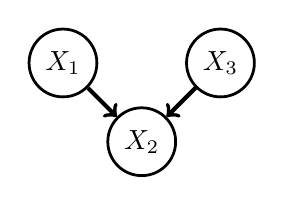
\begin{tikzpicture}[dgraph]
\node[cont] (A) at (0,1) {$X_1$};
\node[cont] (C) at (1,0) {$X_2$};
\node[cont] (B) at (2,1) {$X_3$};
\draw(A) -- (C);\draw(B) -- (C);
\end{tikzpicture}}
\end{center}
$$p(x_1,x_2,x_3) = p(x_2\mid x_1, x_3)p(x_3)p(x_1)$$
\bmp{0.5\tw}
\begin{center}
\begin{tabular}{ccc|c}
$x_2$ & $x_1$ & $x_3$ & $ p(x_2\mid x_3,x_1)$\\ \hline  0 & 0 & 0 & $\theta_1$\\ 0 & 0 & 1& $\theta_2$ \\  0 & 1 & 0 & $\theta_3$ \\  0 & 1 & 1 & $\theta_4$ \\ 
 1 & 0 & 0 & $1 - \theta_1$\\1 & 0 & 1& $1- \theta_2$ \\ 1 & 1 & 0 & $1-\theta_3$ \\ 1 & 1 & 1 & $1-\theta_4$ \\ 
\end{tabular}
\end{center}
\emp
\bmp{0.5\tw}
\begin{center}
\begin{tabular}{c|c}
$x_1$ & $p(x_1)$ \\ \hline  0 & $\theta_5$\\  1 & $1-\theta_5$  \\
\end{tabular}
\end{center}
\begin{center}
\begin{tabular}{c|c}
$x_3$ & $p(x_3)$ \\ \hline  0 & $\theta_6$\\  1 & $1-\theta_6$  \\ 
\end{tabular}
\end{center}
\emp
\end{mybox}
\vspace{0.5cm}
\item \textit{Bayesian Network Examples  }


Solution.
\vspace{0.5cm}

Draw the DAG associated with the following probability distributions:
	\begin{enumerate}
		\item $p(x_1,x_2,x_3) = p(x_2)p(x_3)p(x_2\mid x_1,x_3)$. Show that $X_1 \ci X_3 $.
\begin{center}
\scalebox{0.8}{
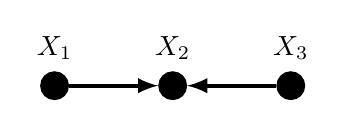
\begin{tikzpicture}[dgraph]
\node[contblk,label=above:{$X_1$}] (x1) at (0,0) {};
\node[contblk, label=above:{$X_2$}] (x2) at (1.5, 0) {};
\node[contblk, label=above:{$X_3$}] (x3) at (3,-0) {};
\draw [-{latex[slant=0]}]  (x1) -- (x2);
\draw [-{latex[slant=0]}] (x3) -- (x2);
\end{tikzpicture}}
\end{center}	
		\item $p(x_1,x_2,x_3) = p(x_1)p(x_2|x_1)p(x_3|x_2)$. Show that $X_1 \ci X_3 | X_2$.		
\begin{center}
\scalebox{0.8}{
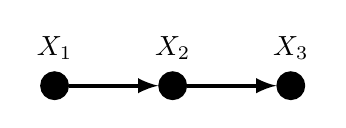
\begin{tikzpicture}[dgraph]
\node[contblk,label=above:{$X_1$}] (x1) at (0,0) {};
\node[contblk, label=above:{$X_2$}] (x2) at (1.5, 0) {};
\node[contblk, label=above:{$X_3$}] (x3) at (3,-0) {};
\draw [-{latex[slant=0]}]  (x1) -- (x2);
\draw [-{latex[slant=0]}] (x2) -- (x3);
\end{tikzpicture}}
\begin{align*}
p(x_1,x_3\mid x_2) &= \frac{p(x_1,x_2,x_3)}{p(x_2)}\\
&= \frac{p(x_1)p(x_2|x_1)p(x_3|x_2)}{p(x_2)}\\
&= \frac{p(x_1,x_2)p(x_3|x_2)}{p(x_2)}\\
&= \frac{p(x_1\mid x_2)p(x_2)p(x_3|x_2)}{p(x_2)}\\
&= p(x_1|x_2)p(x_3|x_2)\\ & \Longrightarrow X_1 \ci X_3 | X_2
\end{align*}
\end{center}		
		\item $p(x_1,x_2,x_3) = p(x_2)p(x_1|x_2)p(x_3|x_2)$. Show that $X_1\ci X_3 | X_2$.		
\begin{center}
\scalebox{0.8}{
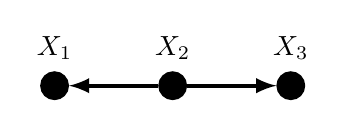
\begin{tikzpicture}[dgraph]
\node[contblk,label=above:{$X_1$}] (x1) at (0,0) {};
\node[contblk, label=above:{$X_2$}] (x2) at (1.5, 0) {};
\node[contblk, label=above:{$X_3$}] (x3) at (3,-0) {};
\draw [-{latex[slant=0]}]  (x2) -- (x1);
\draw [-{latex[slant=0]}] (x2) -- (x3);
\end{tikzpicture}}
\end{center}
\begin{align*}
p(x_1,x_3\mid x_2) &= \frac{p(x_1,x_2,x_3)}{p(x_2)}\\
&= \frac{p(x_2)p(x_1|x_2)p(x_3|x_2)}{p(x_2)}\\
&= p(x_1|x_2)p(x_3|x_2)\\ & \Longrightarrow X_1 \ci X_3 | X_2
\end{align*}		
		\item $p(x_1,x_2,x_3,x_4) = p(x_1)p(x_2)p(x_3|x_1)p(x_4|x_1,x_2)$. Show that $X_3 \ci X_4 | X_1$.
\begin{center}
\scalebox{0.8}{
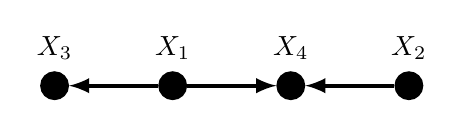
\begin{tikzpicture}[dgraph]
\node[contblk,label=above:{$X_3$}] (x3) at (0,0) {};
\node[contblk, label=above:{$X_1$}] (x1) at (1.5, 0) {};
\node[contblk, label=above:{$X_4$}] (x4) at (3, -0) {};
\node[contblk, label=above:{$X_2$}] (x2) at (4.5,-0) {};
\draw [-{latex[slant=0]}]  (x1) -- (x3);
\draw [-{latex[slant=0]}] (x1) -- (x4);
\draw [-{latex[slant=0]}]  (x2) -- (x4);
\end{tikzpicture}}
\end{center}		
		\item $p(x_1,x_2,x_3,x_4,x_5) = p(x_1)p(x_2)p(x_3|x_1)p(x_4|x_1,x_2)p(x_5|x_4)$. Show that $X_1 \ci X_5 | X_4$.
\begin{center}
\scalebox{0.8}{
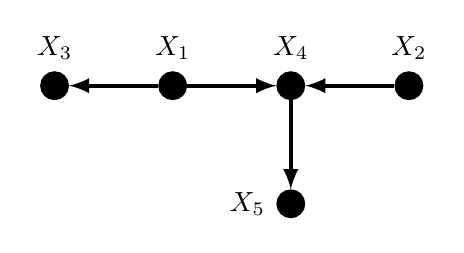
\begin{tikzpicture}[dgraph]
\node[contblk,label=above:{$X_3$}] (x3) at (0,0) {};
\node[contblk, label=above:{$X_1$}] (x1) at (1.5, 0) {};
\node[contblk, label=above:{$X_4$}] (x4) at (3, -0) {};
\node[contblk, label=above:{$X_2$}] (x2) at (4.5,-0) {};
\node[contblk, label=left:{$X_5$}] (x5) at (3,-1.5) {};
\draw [-{latex[slant=0]}]  (x1) -- (x3);
\draw [-{latex[slant=0]}] (x1) -- (x4);
\draw [-{latex[slant=0]}]  (x2) -- (x4);
\draw [-{latex[slant=0]}]  (x4) -- (x5);
\end{tikzpicture}}
\end{center}		
		\item $p(x_1,x_2,x_3,x_4,x_5,x_6) = p(x_1)p(x_2|x_1)p(x_3|x_1)p(x_4|x_2)p(x_5|x_3)p(x_6|x_2,x_5).$ Show that $X_2 \ci X_3 | X_1$.
\begin{center}
\scalebox{0.8}{
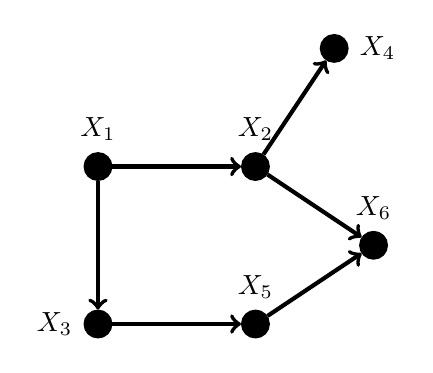
\begin{tikzpicture}[dgraph]
\node[contblk,label=above:{$X_1$}] (x1) at (0,0) {};
\node[contblk,label=above:{$X_2$}] (x2) at (2, 0) {};
\node[contblk,label=left:{$X_3$}] (x3) at (0,-2) {};
\node[contblk,label=right:{$X_4$}] (x4) at (3,1.5) {};
\node[contblk,label=above:{$X_5$}] (x5) at (2,-2) {};
\node[contblk,label=above:{$X_6$}] (x6) at (3.5,-1) {};
\draw(x1) -- (x2);
\draw(x1) -- (x3);
\draw(x2) -- (x4);
\draw(x3) -- (x5);
\draw(x2) -- (x6);
\draw(x5) -- (x6);
\end{tikzpicture}}
\end{center}	

\item Write down the factorization of $p(x_1,x_2,x_3,x_4,x_5,x_6,x_7) $ encoded in the following DAG.
\begin{center}
\scalebox{.9}{
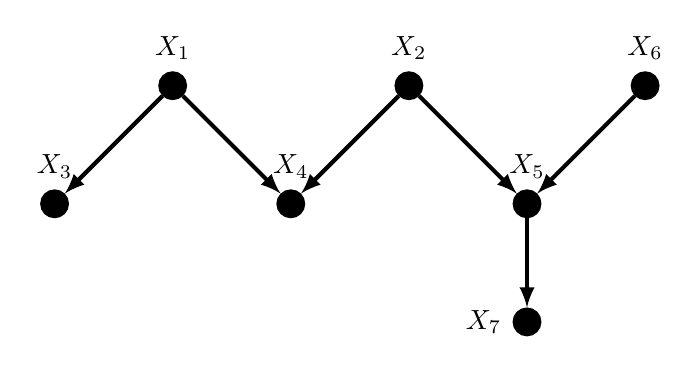
\begin{tikzpicture}[dgraph]
\node[contblk,label=above:{$X_3$}] (x3) at (0,0) {};
\node[contblk, label=above:{$X_1$}] (x1) at (1.5, 1.5) {};
\node[contblk, label=above:{$X_4$}] (x4) at (3, -0) {};
\node[contblk, label=above:{$X_2$}] (x2) at (4.5,1.5) {};
\node[contblk, label=above:{$X_5$}] (x5) at (6, -0) {};
\node[contblk, label=left:{$X_7$}] (x7) at (6, -1.5) {};
\node[contblk, label=above:{$X_6$}] (x6) at (7.5,1.5) {};

\draw [-{latex[slant=0]}]  (x1) -- (x3);
\draw [-{latex[slant=0]}] (x1) -- (x4);
\draw [-{latex[slant=0]}]  (x2) -- (x4);
\draw [-{latex[slant=0]}]  (x2) -- (x5);
\draw [-{latex[slant=0]}]  (x6) -- (x5);
\draw [-{latex[slant=0]}]  (x5) -- (x7);
\end{tikzpicture}}
\end{center}

	\end{enumerate}

\end{itemize}




\begin{mybox}{Application Example (Was it the burglar?) }{theoexample}
 Mary lives in San Francisco City. One afternoon, she is driving back home and receives a phone call from 
 her neighbor Jane. She told her that her house alarm was set off ($\mathsf  A$). While driving, she also heard on the radio
 ($\mathsf  R$) that a small earthquake ($\mathsf  E$) hit the city.  Small earthquakes sometimes activate the alarm, and perhaps
 this is the reason why the alarm was sounding.
 \begin{itemize}
 \item What is the probability that a burglar ($\mathsf B$) broke into the house?
 \item What is the probability that a burglar broke into the house
 given that the alarm was set off?
 \item What is the probability that a burglar broke into the house
 given that the alarm was set off and a small earthquake hit the city?
 \end{itemize} 
\end{mybox}

To solve this problem we make several considerations.
\begin{enumerate}
\item Define the random variables $R(\mathsf R )=1$, $R(\mathsf R^c )=0$, $A(\mathsf A )=1$, $A(\mathsf A^c )=0$,
$E(\mathsf E )=1$, $E(\mathsf E^c )=0$, and $B(\mathsf B )=1$, $B(\mathsf B^c )=0$.
\item Assume that the joint distribution of random variables $R$, $A$, $E$, and $B$ factorizes as 
 $$\small p(R,A,E,B)=p(E=e)p(B=b)p(A=a\mid B=b,E=e)p(R=r\mid E=e)$$ our using our simplified 
notation
 $$p(r,a,e,b)=p(e)p(b)p(a\mid b,e)p(r\mid e).$$
\end{enumerate}




The factors of the probability distribution correspond to the following tables.
 
  \bmp{0.4\tw}  
  \begin{center}
  \begin{tabular}{l l l }
    \hline
            & $b$ & $p(b)$ \\\hline\hline
     $\mathsf{B^c}$ & $\mathsf 0$ & $\mathsf{b_1 = .9}$\\
     $\mathsf{B}$    &  $\mathsf 1$ & $1-\mathsf{b_1}$\\     
     \hline
  \end{tabular}
  
  \vspace{0.2cm}
  \begin{tabular}{l l l }
    \hline
            & $e$ & $p(e)$ \\\hline\hline
     $\mathsf{E^c}$ & $\mathsf 0$ & $\mathsf{e_1 = 0.95}$\\
     $\mathsf{E}$    &  $\mathsf 1$ & $\mathsf{e_2}$ \\     
     \hline
  \end{tabular}
    \vspace{0.2cm}
  \begin{tabular}{l l l }
    \hline
            & $r$ & $p(r)$ \\\hline\hline
     $\mathsf{R^c}$ & $\mathsf 0$ & $\mathsf{c_1 = 0.05}$\\
     $\mathsf{R}$    &  $\mathsf 1$ & $\mathsf{c_2}$\\     
     \hline
  \end{tabular}  
\end{center}
\emp
 \bmp{0.6\tw}  
  \begin{center}
  \begin{tabular}{l l l l l}
    \hline
                              &                           & $b$  & $e $ & $p(b,e)$ \\\hline\hline
     $\mathsf{B^c}$ &  $\mathsf{E^c}$ &  $\mathsf 0$     &   $\mathsf 0$    &  $\mathsf{b_1e_1}$\\
     $\mathsf{B^c}$ &  $\mathsf{E}$    &  $\mathsf 0$     &   $\mathsf 1$    &  $\mathsf{b_1e_2}$\\  
     $\mathsf{B}$    &  $\mathsf{E^c}$ &  $\mathsf 1$     &   $\mathsf 0$    &  $\mathsf{b_2e_1}$\\
     $\mathsf{B}$.   &  $\mathsf{E}$    &  $\mathsf 1$        &   $\mathsf 1$    &  $\mathsf{b_2e_2}$\\     
        
     \hline
  \end{tabular}
\end{center}
  \begin{center}
  \begin{tabular}{l l l l l}
    \hline
                              &                           & $r$  & $e $ & $p(r\mid e)$ \\\hline\hline
     $\mathsf{R^c}$ &  $\mathsf{E^c}$ &  $\mathsf 0$     &   $\mathsf 0$    &  $\mathsf f_1=0.99$\\
     $\mathsf{R^c}$ &  $\mathsf{E}$    &  $\mathsf 0$     &   $\mathsf 1$    &  $\mathsf f_2=0.01$\\  
     $\mathsf{R}$    &  $\mathsf{E^c}$ &  $\mathsf 1$     &   $\mathsf 0$    &  $\mathsf{f_3=1-f_1}$\\
     $\mathsf{R}$.   &  $\mathsf{E}$    &  $\mathsf 1$        &   $\mathsf 1$    &  $\mathsf {f_4=1-f_2}$\\     
        
     \hline
  \end{tabular}
\end{center}
\emp
\vspace{0.5cm}

   \bmp{0.6\tw}  
  \begin{center}
  \begin{tabular}{l l l l  l l l l l }
    \hline
               &       &     &  $ { a}$ & $ { b}$ & $ { e}$ &$ p(a\mid b,e)$ \\ \hline\hline
     $\mathsf{A^c}$ & $\mathsf{B^c}$ & $\mathsf{E^c}$   & $ \mathsf{ 0}$ & $\mathsf {0}$ & $  \mathsf {0}$ &$ \mathsf{q_1}$ \\ %\hline
     $\mathsf{A^c}$ & $\mathsf{B^c}$ & $\mathsf{E}$    & $ \mathsf{0}$ & $\mathsf {0}$ & $  \mathsf {1}$ &  $  \mathsf{q_2}$ \\ %\hline
     $\mathsf{A^c}$ & $\mathsf{B}$ & $\mathsf{E^c}$     & $\mathsf{ 0}$ & $\mathsf {1}$ & $ \mathsf {0}$ &  $ \mathsf{q_3}$ \\ %\hline
     $\mathsf{A^c}$ & $\mathsf{B}$ & $\mathsf{E}$    & $ \mathsf{ 0}$ & $\mathsf{1}$ & $  \mathsf{1}$ &  $ \mathsf{q_4}$ \\ %\hline
     $\mathsf{A}$ & $\mathsf{B^c}$ & $\mathsf{E^c}$     & $ \mathsf{ 1}$ & $\mathsf {0}$ & $  \mathsf {0}$ &  $  \mathsf{q_5}$\\ %\hline
     $\mathsf{A}$ & $\mathsf{B^c}$ & $\mathsf{E}$    & $ \mathsf{ 1}$ & $\mathsf {0}$ & $  \mathsf{1}$ &  $ \mathsf{q_6}$ \\ %\hline
     $\mathsf{A}$ & $\mathsf{B}$ & $\mathsf{E^c}$     & $ \mathsf{ 1}$ & $\mathsf{1}$ & $ \mathsf {0}$ &  $  \mathsf{q_7}$ \\ %\hline
     $\mathsf{A}$ & $\mathsf{B}$ & $\mathsf{E}$     & $ \mathsf{ 1}$ & $\mathsf{1}$ & $  \mathsf{1}$ &  $  \mathsf{q_8}$ \\ %\hline
    \hline
  \end{tabular}
\end{center}
\emp
\bmp{0.4\tw}  
  \begin{center}
  
$\mathsf {q_1+q_5 = 1}$,  $\mathsf {q_2+q_6 = 1}$, $\mathsf {q_3+q_5 = 1}$, $\mathsf {q_4+q_8 = 1}$, $\mathsf {b_1+b_2=1}$, $\mathsf {e_1+e_2=1}$, $\mathsf {c_1+c_2=1}$,
 
$\mathsf{f_1+f_3=1}$, 

$\mathsf{f_2+f_4 = 1}$.

\end{center}
\emp

\vspace{0.5cm}

The table representing the joint probability function is 
\vspace{0.5cm}

   \bmp{0.7\tw}  
  \begin{center}
  \begin{tabular}{l l l l  l l l l l }
    \hline
        &       &       &     &  $ {  r}$ & $ { a}$ & $ { b}$ & $ { e}$ &$ p(r,a,e,b)$ \\ \hline\hline
   $\mathsf{R^c}$ & $\mathsf{A^c}$ & $\mathsf{B^c}$ & $\mathsf{E^c}$ &  $ \mathsf{ 0}$ & $ \mathsf{ 0}$ & $\mathsf {0}$ & $  \mathsf {0}$ &$ \mathsf{p_1}=     \mathsf{b_1e_1f_1p_1}$ \\ %\hline
   $\mathsf{R^c}$ & $\mathsf{A^c}$ & $\mathsf{B^c}$ & $\mathsf{E}$ &  $ \mathsf{ 0}$  & $ \mathsf{0}$ & $\mathsf {0}$ & $  \mathsf {1}$ &  $  \mathsf{p_2}=    \mathsf{b_1e_2f_1p_2}$ \\ %\hline
   $\mathsf{R^c}$ & $\mathsf{A^c}$ & $\mathsf{B}$ & $\mathsf{E^c}$ &  $ \mathsf{ 0}$  & $\mathsf{ 0}$ & $\mathsf {1}$ & $ \mathsf {0}$ &  $ \mathsf{p_3}=     \mathsf{b_2e_1f_1p_3}$ \\ %\hline
   $\mathsf{R^c}$ & $\mathsf{A^c}$ & $\mathsf{B}$ & $\mathsf{E}$ &  $\mathsf{ 0}$  & $ \mathsf{ 0}$ & $\mathsf{1}$ & $  \mathsf{1}$ &  $ \mathsf{p_4}=      \mathsf{b_2e_2f_1p_4}$ \\ %\hline
   $\mathsf{R^c}$ & $\mathsf{A}$ & $\mathsf{B^c}$ & $\mathsf{E^c}$ &  $\mathsf{ 0}$  & $ \mathsf{ 1}$ & $\mathsf {0}$ & $  \mathsf {0}$ &  $  \mathsf{p_5}=     \mathsf{b_1e_1f_2p_5}$\\ %\hline
   $\mathsf{R^c}$ & $\mathsf{A}$ & $\mathsf{B^c}$ & $\mathsf{E}$ &  $\mathsf{ 0}$  & $ \mathsf{ 1}$ & $\mathsf {0}$ & $  \mathsf{1}$ &  $ \mathsf{p_6}=     \mathsf{b_1e_2f_2p_6}$ \\ %\hline
   $\mathsf{R^c}$ & $\mathsf{A}$ & $\mathsf{B}$ & $\mathsf{E^c}$ &  $\mathsf{ 0}$  & $ \mathsf{ 1}$ & $\mathsf{1}$ & $ \mathsf {0}$ &  $  \mathsf{p_7}=      \mathsf{b_2e_1f_2p_7}$ \\ %\hline
   $\mathsf{R^c}$ & $\mathsf{A}$ & $\mathsf{B}$ & $\mathsf{E}$ &  $\mathsf{0}$   & $ \mathsf{ 1}$ & $\mathsf{1}$ & $  \mathsf{1}$ &  $  \mathsf{p_8}=       \mathsf{b_2e_2f_2p_8}$ \\ %\hline
   $\mathsf{R}$ & $\mathsf{A^c}$ & $\mathsf{B^c}$ & $\mathsf{E^c}$ &  $ \mathsf{1}$  & $ \mathsf{ 0}$ & $\mathsf {0}$ & $ \mathsf {0}$ &  $ \mathsf{p_9}=     \mathsf{b_1e_1f_3p_1}$ \\ %\hline
   $\mathsf{R}$ & $\mathsf{A^c}$ & $\mathsf{B^c}$ & $\mathsf{E}$ &  $\mathsf{ 1}$  & $ \mathsf{ 0}$ & $\mathsf {0}$ & $  \mathsf{1}$ &  $  \mathsf{p_{10}}= \mathsf{b_1e_2f_3p_2}$ \\ %\hline
   $\mathsf{R}$ & $\mathsf{A^c}$ & $\mathsf{B}$ & $\mathsf{E^c}$ &  $\mathsf{ 1}$  & $ \mathsf{ 0}$ & $\mathsf{1}$ & $ \mathsf {0}$ &  $  \mathsf{p_{11}}=  \mathsf{b_2e_1f_3p_3}$ \\ %\hline
   $\mathsf{R}$ & $\mathsf{A^c}$ & $\mathsf{B}$ & $\mathsf{E}$ &  $\mathsf{ 1}$  & $ \mathsf{ 0}$ & $\mathsf{1}$ & $ \mathsf {1}$ &  $  \mathsf{p_{12}}=  \mathsf{b_2e_2f_3p_4}$ \\ %\hline
   $\mathsf{R}$ & $\mathsf{A}$ & $\mathsf{B^c}$ & $\mathsf{E^c}$ &  $\mathsf{ 1}$  & $ \mathsf{ 1}$ & $\mathsf{0}$ & $ \mathsf {0}$ &  $ \mathsf{p_{13}}=  \mathsf{b_1e_1f_4p_5}$ \\ %\hline
   $\mathsf{R}$ & $\mathsf{A}$ & $\mathsf{B^c}$ & $\mathsf{E}$ &  $\mathsf{ 1}$  & $ \mathsf{ 1}$ & $\mathsf{0}$ & $ \mathsf {1}$ &  $  \mathsf{p_{14}}=  \mathsf{b_1e_2f_4p_6}$ \\ %\hline
   $\mathsf{R}$ & $\mathsf{A}$ & $\mathsf{B}$ & $\mathsf{E^c}$ &  $\mathsf{ 1}$  & $ \mathsf{ 1}$ & $\mathsf{1}$ & $ \mathsf {0}$ &  $ \mathsf{p_{15}}=  \mathsf{b_2e_1f_4p_7}$ \\ %\hline
   $\mathsf{R}$ & $\mathsf{A}$ & $\mathsf{B}$ & $\mathsf{E}$ &  $\mathsf{ 1}$  & $ \mathsf{ 1}$ & $\mathsf{1}$ & $ \mathsf {1}$ &  $  \mathsf{p_{16}}=  \mathsf{b_2e_2f_4p_8}$ \\ %\hline

    \hline
  \end{tabular}
\end{center}
\emp
\bmp{0.3\tw}  
  \begin{center}
  
$\mathsf {q_1+q_5 = 1}$,  $\mathsf {q_2+q_6 = 1}$, $\mathsf {q_3+q_5 = 1}$, $\mathsf {q_4+q_8 = 1}$, $\mathsf {b_1+b_2=1}$, $\mathsf {e_1+e_2=1}$, $\mathsf {c_1+c_2=1}$, $f_1+f_3=1$, 
$f_2+f_4 = 1$.

\end{center}
\emp  

\begin{marginfigure}
\centering
\begin{center}
\scalebox{.9}{
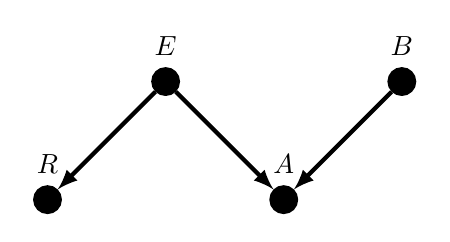
\begin{tikzpicture}[dgraph]
\node[contblk,label=above:{$R$}] (x3) at (0,0) {};
\node[contblk, label=above:{$E$}] (x1) at (1.5, 1.5) {};
\node[contblk, label=above:{$A$}] (x4) at (3, -0) {};
\node[contblk, label=above:{$B$}] (x2) at (4.5,1.5) {};
\draw [-{latex[slant=0]}]  (x1) -- (x3);
\draw [-{latex[slant=0]}] (x1) -- (x4);
\draw [-{latex[slant=0]}]  (x2) -- (x4);
\end{tikzpicture}}
\end{center}
\caption{Directed Acyclic Graph encoding the 
probability distribution $p(r,a,e,b)=p(e)p(b)p(a\mid b,e)p(r\mid e).$ Dark circles represent random variables $R$, $A$, $E$, and $B$. 
}

\end{marginfigure}

\vspace{0.5cm}

\begin{itemize}
\item The \textit{graphical model}  (a Directed Acyclic Graph or DAG) encoding the 
probability distribution factorization is shown in Figure 21.
\item Assume that  $q_1=0.98$, $q_2=0.9$, $q_3=0.1$, $q_4=0.01$.
\item What is the probability that a burglar broke into the house?
\begin{align*}
P(B=\mathsf 1) &= P(\mathsf{B}) = \\ &= \mathsf{ p_3+p_4+p_7+p_8+p_{11}+p_{12}+p_{15}+p_{16},}
\end{align*}
\begin{align*}
P(B=\mathsf 1) &= \sum_{a}\sum_{r}\sum_{e} p(r,a,B=1,e) = 0.1.
\end{align*}
%\item What is the computational complexity of computing $p(B)$?
\end{itemize}

\begin{itemize}
\item What is the probability that a burglar broke into the house
 given that the alarm was set off?
\begin{align*}
P(B=\mathsf 1\mid A=1) &= \frac{P(B=1,A=1 )}{P(A=1)}\\ &= \frac{\mathsf{ p_{7}+p_{8}+p_{15}+p_{16}}}{\mathsf{p_{5}+p_{6}+p_{7}+p_{8}+p_{13}+p_{14}+p_{15}+p_{16}}},
\end{align*}
\begin{align*}
P(B=\mathsf 1\mid A=1) &= \frac{\sum_{r}\sum_{e} p(r,A=1,B=1,e)}{\sum_{r}\sum_{b}\sum_{e} p(r,A=1,b,e) } &= 0.81.
\end{align*}
\end{itemize}

\begin{itemize}
\item What is the probability that a burglar broke into the house
 given that the alarm was set off and a small earthquake hit the city?
\begin{align*}
P(B=\mathsf 1\mid A=1, E=1) &= \frac{P(B=1,A=1,E=1 )}{P(A=1,E=1)}\\ &= \frac{\mathsf{p_{8} +p_{16}}}{\mathsf{p_{6}+ p_{8}+p_{14}+p_{16}}},
\end{align*}
\begin{align*}
P(B=\mathsf 1\mid A=1,E=1) &= \frac{\sum_{r}p(r,A=1,B=1,E=1)}{\sum_{r}\sum_{b} p(r,A=1,b,E=1) } \\&= 0.51.
\end{align*}
\end{itemize}

\begin{mybox}{Solution Summary }{theoexample}
\begin{itemize}
 \item What is the probability that a burglar broke into the house?
 \begin{align*}
P(B=\mathsf 1) &= 0.1.
\end{align*}
 \item What is the probability that a burglar broke into the house
 given that the alarm was set off?
 \begin{align*}
P(B=\mathsf 1\mid A=1) &= 0.81.
\end{align*}
 \item What is the probability that a burglar broke into the house given that the alarm was set off and a small earthquake hit the city?
 \begin{align*}
P(B=\mathsf 1\mid A=1,E=1) &= 0.51.
\end{align*}
\item The \textit{a priori} probability that the burglar broke into the house is $0.1$. The probability that a burglar broke into the house
 given that the alarm was set off is much higher  ($0.81$). However, knowing that a small earthquake hit the city \textit{explains away} the observation that the alarm was set off,
 diminishing the probability that a burglar broke ($0.51$). 
 \end{itemize} 
\end{mybox}
\begin{itemize}
 \item Note that the factorization features of the probability distribution and the sum-product distributive property help us reduce the computational complexity. 
 \begin{align*}
 p(b\mid a) = \frac{p(a,b)}{p(a)} &= \frac{\sum_r\sum_ep(r,a,e,b)}{\sum_b\sum_r\sum_ep(r,a,e,b)}\\
 					       &= \frac{\sum_r\sum_e p(e)p(b)p(a\mid e,b)p(r\mid e)}{\sum_b\sum_r\sum_e p(e)p(b)p(a\mid e,b)p(r\mid e)}\\
                                                 &= \frac{p(b)\sum_e p(e)p(a\mid e,b)\sum_rp(r\mid e)}{\sum_bp(b)\sum_e p(e)p(a\mid e,b)\sum_rp(r\mid e)}\\
                                                 &= \frac{p(b)\sum_e p(e)p(a\mid e,b)\phi_1(e)}{\sum_b p(b)\sum_e p(e)p(a\mid e,b)\phi_1(e)}\\
                                                  &= \frac{p(b)\phi_2(a,b)}{\sum_b p(b)\phi_2(a,b)}\\
                                                 &= \frac{p(b)\phi_2(a,b)}{\phi_3(a)}\\
 \end{align*}
\end{itemize}


\subsection{Generic table}
\vspace{0.2cm}  
  \bmp{0.5\tw}  
\begin{center}
 \begin{tabular}{l l l l  l l l l l }
\hline
& & & & $d$& $b$& $a$& $c$ & $p(d,b,a,c)$ \\\hline\hline
$\mathsf D^\mathsf c$& $\mathsf B^ \mathsf c$ & $\mathsf A^ \mathsf c$ & $\mathsf C^ \mathsf c$ &  $\mathsf 0$  & $\mathsf 0$  & $\mathsf 0$  & $\mathsf 0$   & $\mathsf{p_0    =  c_1a_1b_1d_1}$\\ %\hline
$\mathsf D^\mathsf c$& $\mathsf B^\mathsf c$ & $\mathsf A^ \mathsf c$ & $\mathsf C  $ &  $\mathsf 0$  & $\mathsf 0$  & $\mathsf 0$  & $\mathsf 1$   & $\mathsf{p_1     =  c_2a_2b_1d_2}$ \\ %\hline
$\mathsf D^ \mathsf c$& $\mathsf B^\mathsf c$ & $\mathsf A  $ & $\mathsf C^\mathsf c$ &  $\mathsf 0$  & $\mathsf 0$  & $\mathsf 1$  & $\mathsf 0$   & $\mathsf{p_2     =  c_1a_1b_1d_1}$ \\ %\hline
$\mathsf D^ \mathsf c$& $\mathsf B^ \mathsf c$ & $\mathsf A  $ & $\mathsf C  $ &  $\mathsf 0$  & $\mathsf 0$  & $\mathsf 1$  & $\mathsf 1$   & $\mathsf{p_3      =  c_2a_2b_1d_2}$ \\ %\hline
$\mathsf D^\mathsf c$& $\mathsf B  $ & $\mathsf A^c$ & $\mathsf C^\mathsf c$ &  $\mathsf 0$  & $\mathsf 1$  & $\mathsf 0$  & $\mathsf 0$   & $\mathsf{p_4    =  c_1a_1b_2d_1}$ \\ %\hline
$\mathsf D^\mathsf c$& $\mathsf B  $ & $\mathsf A^c$ & $\mathsf C  $ &  $\mathsf 0$  & $\mathsf 1$  & $\mathsf 0$  & $\mathsf 1$   & $\mathsf{p_5     =  c_2a_2b_2d_2}$ \\ %\hline
$\mathsf D^\mathsf c$& $\mathsf B  $ & $\mathsf A  $ & $\mathsf C^ \mathsf c$ &  $\mathsf 0$  & $\mathsf 1$  & $\mathsf 1$  & $\mathsf 0$   & $\mathsf{p_6     =  c_1a_1b_2d_1}$ \\ %\hline
$\mathsf D^\mathsf c$& $\mathsf B  $ & $\mathsf A  $ & $\mathsf C  $ &  $\mathsf 0$  & $\mathsf 1$  & $\mathsf 1$  & $\mathsf 1$   & $\mathsf{p_7      =  c_2a_2b_2d_2}$ \\ %\hline
$\mathsf D  $& $\mathsf B^\mathsf c$ & $\mathsf A^ \mathsf c$ & $\mathsf C^\mathsf c$ &  $\mathsf 1$  & $\mathsf 0$  & $\mathsf 0$  & $\mathsf 0$   & $\mathsf{p_8   =  c_1a_1b_1d_3}$ \\ %\hline
$\mathsf D  $& $\mathsf B^\mathsf c$ & $\mathsf {A ^c}$ & $\mathsf C  $ &  $\mathsf 1$  & $\mathsf 0$  & $\mathsf 0$  & $\mathsf 1$   & $\mathsf{p_9    =  c_2a_2b_1d_4}$ \\ %\hline
$\mathsf D  $& $\mathsf B^\mathsf c$ & $\mathsf A  $ & $\mathsf C^\mathsf c$ &  $\mathsf 1$  & $\mathsf 0$  & $\mathsf 1$  & $\mathsf 0$   & $\mathsf{p_{10}=  c_1a_1b_1d_3}$ \\ %\hline
$\mathsf D  $& $\mathsf B^\mathsf c$ & $\mathsf A  $ & $\mathsf C  $ &  $\mathsf 1$  & $\mathsf 0$  & $\mathsf 1$  & $\mathsf 1$   & $\mathsf{p_{11}  =  c_2a_2b_1d_4}$ \\ %\hline
$\mathsf D  $& $\mathsf B  $ & $\mathsf A^\mathsf c$ & $\mathsf C^\mathsf c$ &  $\mathsf 1$  & $\mathsf 1$  & $\mathsf 0$  & $\mathsf 0$   & $\mathsf{p_{12}=  c_1a_1b_2d_3}$\\ %\hline
$\mathsf D  $& $\mathsf B  $ & $\mathsf A^\mathsf c$ & $\mathsf C  $ &  $\mathsf 1$  & $\mathsf 1$  & $\mathsf 0$  & $\mathsf 1$   & $\mathsf{p_{13}  = c_2a_2b_2d_4}$ \\ %\hline
$\mathsf D  $& $\mathsf B  $ & $\mathsf A  $ & $\mathsf C^\mathsf c$ &  $\mathsf 1$  & $\mathsf 1$  & $\mathsf 1$  & $\mathsf 0$   & $\mathsf{p_{14}  = c_1a_1b_2d_3}$ \\ %\hline
$\mathsf D  $& $\mathsf B  $ & $\mathsf A  $ & $\mathsf C  $ &  $\mathsf 1$  & $\mathsf 1$  & $\mathsf 1$  & $\mathsf 1$   & $\mathsf{p_{15}   =  c_2a_2b_2d_4}$ \\ %\hline
\end{tabular}
\end{center}
 \emp


\begin{marginfigure}
\centering
\begin{center}
\scalebox{.9}{
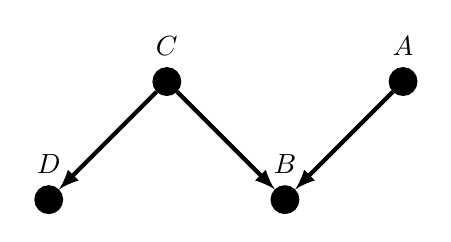
\begin{tikzpicture}[dgraph]
\node[contblk,label=above:{$D$}] (x3) at (0,0) {};
\node[contblk, label=above:{$C$}] (x1) at (1.5, 1.5) {};
\node[contblk, label=above:{$B$}] (x4) at (3, -0) {};
\node[contblk, label=above:{$A$}] (x2) at (4.5,1.5) {};
\draw [-{latex[slant=0]}]  (x1) -- (x3);
\draw [-{latex[slant=0]}] (x1) -- (x4);
\draw [-{latex[slant=0]}]  (x2) -- (x4);
\end{tikzpicture}}
\end{center}
\caption{Directed Acyclic Graph encoding the 
probability distribution $p(d,b,a,c)=p(c)p(a)p(b\mid a,c)p(d\mid c).$ Dark circles represent random variables $D$, $B$, $A$, and $C$. 
}

\end{marginfigure}


\begin{mybox}{Application Example (Pairs of dice) }{theoexample}
\small
You are told that there are two pairs of coins. The first pair is fair, $$\theta_1(\mathsf H)=\theta_1(\mathsf T)=\frac{1}{2}.$$ The second pair is biased as both coins have probability $$\theta_2(\mathsf H)=\frac{2}{3},\,\, \theta_2(\mathsf T)=\frac{1}{3}$$  of producing heads  and  tails, respectively. One of the two pairs is chosen at random with probability 0.5 and thrown 10 times. The sum of the coins is recorded for each throw.
 \begin{enumerate}
\item If the throw results in the sequence "1010101010"? Which pair of dice was picked for the throw?
\item Repeat (1) for the sequence "2222200000". 
\item Assume that the result of the second coin is flipped ($\mathsf F$) with probability $\sf p=0.5$ before recording the result of the throw with probability. Repeat  1 and 2 under this assumption. Consider the case for which  $\sf p = 0.2$. Repeat exercises 1 and 2.
\vspace{0.2cm}

\noindent The graphical model associated with this problem is as follows.

\begin{center}
\scalebox{0.8}{
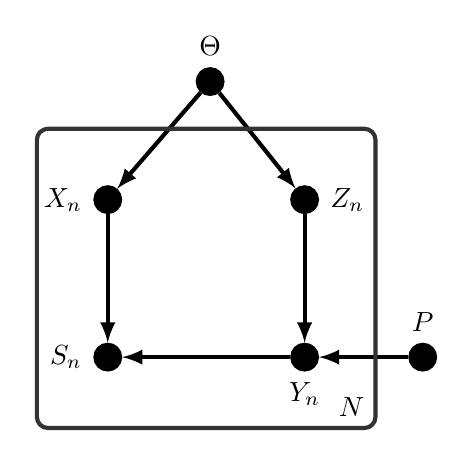
\begin{tikzpicture}[dgraph]
\node[contblk,label=above:{$\Theta$}] (theta) at (2.3,1.5) {};
\node[contblk, label=left:{$X_n$}] (xn) at (1, 0) {};
\node[contblk, label=right:{$Z_n$}] (zn) at (3.5, 0) {};
\node[contblk, label=below:{$Y_n$}] (yn) at (3.5,-2) {};
\node[contblk, label=left:{$S_n$}] (sn) at (1,-2) {};
\node[contblk, label=above:{$P$}] (p) at (5.0,-2) {};
\draw [-{latex[slant=0]}]  (theta) -- (xn);
\draw [-{latex[slant=0]}] (theta) -- (zn);
\draw [-{latex[slant=0]}]  (zn) -- (yn);
\draw [-{latex[slant=0]}]  (xn) -- (sn);
\draw [-{latex[slant=0]}]  (yn) -- (sn);
\draw [-{latex[slant=0]}]  (p) -- (yn);
\boxit{$N$}{(sn)}{(zn)}{0.9};
\end{tikzpicture}}
\end{center}
\end{enumerate}
\begin{itemize}
\item $X_n$ represents the $n$-th result from the throw of the first coin; $X_n(\sf H) = 1$ and $X_n(\sf T) = 0$, and
$$p(x_n\mid \theta) = \theta^{x_n}(1-\theta)^{(1-x_n)}. $$ 
\item $Z_n$ epresents the unobserved   result from the $n$-th throw of the second coin;  $Z_n(\sf F) = 1$ and $Z_n(\sf F^c) = 0$, and
$$p(z_n\mid \theta) = \theta^{z_n}(1-\theta)^{(1-z_n)}. $$
\item $Y_n$ represents the recorded result  from the $n$-th throw of the second coin; $Y_n(\sf H) = 1$ and $Y_n(\sf T) = 0$, and 
$$p(y_n\mid z_n, p) = p^{I(y_n \neq z_n)} (1-p)^{ I(y_n = z_n)}.$$
\item $S_n$ is a deterministic function of $X_n$ and $Y_n$,  $$S_n=X_n+Y_n,$$ $$p(s_n\mid x_n, y_n) = \mathrm I(s_n == x_n+y_n),$$ and
\begin{equation*}
 I(e) =
    \begin{cases}
      1, & \textrm{if}\,\,e = \mathsf{true};\\
      0, & \textrm{otherwise}.\\
    \end{cases}       
\end{equation*}
 
\end{itemize}
\end{mybox}

Let  $\mathbf X = (X_1,X_2, \dots, X_N)$,  $\mathbf Y = (Y_1,Y_2, \dots, Y_N)$,  $\mathbf Z = (Z_1,Z_2, \dots, Z_N)$,
$\mathbf S = (S_1,S_2, \dots, S_N)$, $f_n= I(y_n \neq z_n) = 1 - I(y_n = z_n)$, and $\mathbf f = (f_1,f_2, \dots, f_N)$. ($f_n$ indicates whether the second was flipped or not.) 
The joint probability distribution for  $\mathbf x, \mathbf z, \mathbf y, \mathbf s $ given $\theta$ and $p$ is

\begin{align*}
p(\mathbf x, \mathbf z, \mathbf y, \mathbf s, \theta,  p) &= p(\theta)p(p)\prod_{n=1}^{N} p(x_n\mid \theta)p(z_n\mid \theta)p(y_n\mid z_n, p) p(s_n \mid x_n,y_n)\\
p(\mathbf x, \mathbf z, \mathbf y, \mathbf s \mid \theta,  p) &= \frac{p(\mathbf x, \mathbf z, \mathbf y, \mathbf s, \theta,  p)}{p(\theta)p(p)}\\
p(\mathbf x, \mathbf z, \mathbf y, \mathbf s \mid \theta,  p)  &= \prod_{n=1}^{N} p(x_n\mid \theta)p(z_n\mid \theta)p(y_n\mid z_n, p) p(s_n \mid x_n,y_n)\\
&=  \prod_{n=1}^{N}  \theta^{x_n}(1-\theta)^{(1-x_n)}  \theta^{z_n}(1-\theta)^{(1-z_n)} p^{I(y_n \neq z_n)} (1-p)^{ I(y_n = z_n)}  I(s_n = x_n + y_n).\\
&=  \theta^{\sum_{n=1}^N x_n}(1-\theta)^{\sum_{n=1}^N(1-x_n)}  \theta^{\sum_{n=1}^N z_n}(1-\theta)^{\sum_{n=1}^N(1-z_n)} p^{\sum_{n=1}^N I(y_n \neq z_n)} (1-p)^{ \sum_{n=1}^N I(y_n = z_n)} \\
\end{align*}

Notice that 

$$x_n = s_n - y_n,$$
$$y_n = z_n(1-f_n)+(1-z_n)f_n,$$ and
$$x_n = s_n - z_n + 2z_nf_n - f_n.$$

We define $N_x$, and $N_z$ as follows,

$$ N_x = \sum_{n=1}^{N} (s_n - z_n + 2z_nf_n - f_n) = N_s - N_z + 2N_{zf}-N_f  \geq 0,$$
$$ N_s = \sum_{n=1}^{N} s_n,$$
$$ N_z = \sum_{n=1}^{N} z_n,$$
$$ N_{zf} = \sum_{n=1}^{N} z_nf_n,$$and
$$N_f = \sum_{n=1}^{N} f_n.$$

Therefore we can write the probability distribution function as follows,
\begin{align*}
p(\mathbf x, \mathbf z, \mathbf y, \mathbf s \mid \theta,  p) &=  \theta^{\sum_{n=1}^N x_n}(1-\theta)^{\sum_{n=1}^N(1-x_n)}  \theta^{\sum_{n=1}^N z_n}(1-\theta)^{\sum_{n=1}^N(1-z_n)} p^{\sum_{n=1}^N f_n} (1-p)^{ \sum_{n=1}^N (1-f_n)} \\
&=  \theta^{N_x}(1-\theta)^{(N-N_x)} \theta^{N_z}(1-\theta)^{(N-N_z)}p^{N_f}(1-p)^{N-N_f}\\
&=  \theta^{N_x + N_z }(1-\theta)^{(2N-(N_x+N_z))} p^{N_f}(1-p)^{N-N_f}\\
&= p(\mathbf s, \mathbf z, \mathbf f \mid \theta, p)
\end{align*}
Observe  that 
$N_x = N_x(\mathbf s,\mathbf z, \mathbf f),$
$N_z = N_z(\mathbf z),$ and therefore

$$ p(\mathbf x, \mathbf z, \mathbf y, \mathbf s \mid \theta, p) =  p(\mathbf s, \mathbf z, \mathbf f \mid \theta, p). $$  Also,

$$ p(\mathbf s \mid \theta, p) =  \sum_{\mathbf x}  \sum_{\mathbf z} \sum_{\mathbf y} p(\mathbf x, \mathbf z, \mathbf y, \mathbf s \mid \theta, p) =  \sum_{\mathbf f} \sum_{\mathbf z} p(\mathbf s, \mathbf z, \mathbf f \mid \theta, p),$$ and

\begin{align*}
p(\theta\mid \mathbf s, p) &= \frac{p(\mathbf s, \theta, p)}{p( \mathbf s, p)}= \frac{p(\mathbf s\mid \theta, p)p(\theta,p)}{p( \mathbf s, p)} \\
                                         &=  \frac{p(\mathbf s\mid \theta, p)p(\theta\mid p)p(p)}{p( \mathbf s\mid p)p(p)}\\
                                         &=  \frac{p(\mathbf s\mid \theta, p)p(\theta\mid p)}{p( \mathbf s\mid p)}\\
                                         &=  \frac{p(\mathbf s\mid \theta, p)p(\theta)}{p( \mathbf s\mid p)}. 
\end{align*}
since $\theta \ci p$.

 \begin{mybox}{Decision Rule }{theoexample}

$$ \mathrm I\left(\frac{p(\theta_1 \mid ,\mathbf s,  p)}  {p(\theta_2 \mid ,\mathbf s,  p)} > 1 \right)  \Rightarrow \text{choose $ \theta_1$},$$ 
which is equivalent to
$$ \mathrm I\left(\frac{p(\mathbf s \mid \theta_1, p)p(\theta_1)}  {p(\mathbf s \mid \theta_2, p)p(\theta_2)} > 1 \right)  \Rightarrow \text{choose $ \theta_1$},$$ 
since
$$p(\theta \mid ,\mathbf s,  p) \propto  p(\mathbf s \mid \theta, p)p(\theta) =    \sum_{\mathbf f} \sum_{\mathbf z} p(\mathbf s, \mathbf z, \mathbf f \mid \theta, p) p(\theta).$$

Notice that 

$$ p(\mathbf s|p) = \sum_{\theta} \sum_{\mathbf f} \sum_{\mathbf z} p(\mathbf s, \mathbf z, \mathbf f \mid \theta, p)p(\theta),$$ with $\theta \in \{\theta_1,\theta_2\}.$

\end{mybox}

\begin{marginfigure}
\centering
\includegraphics[width=4cm]{fig/12.png}
\caption{Probability distribution $p(N_s)$ in Box for $\theta= \frac{1}{2}$ for problem 3 in Box 9.
The expected value $\mu_{N_s}= 5$ and the entropy is $E(N_s)=2.71$.
}
\end{marginfigure}




These equations lead to the following results regarding question 3.

\begin{align*}
\frac{p([2, 2, 2, 2, 2, 0, 0, 0, 0, 0]\mid \frac{2}{3}, \frac{1}{2})p(\frac{2}{3})}{p([2, 2, 2, 2, 2, 0, 0, 0, 0, 0]\mid  \frac{1}{2}, \frac{1}{2})p(\frac{1}{2})} &= 1.80 \Longrightarrow  \theta_2 = \frac{2}{3}.\\
\frac{p([1,0,1,0,1,0,1,0,1,0]\mid \frac{2}{3}, \frac{1}{2})p(\frac{2}{3})}{p([1,0,1,0,1,0,1,0,1,0]\mid  \frac{1}{2}, \frac{1}{2})p(\frac{1}{2})} &= 0.13 \Longrightarrow  \theta_1 = \frac{1}{2}. 
\end{align*}

\begin{figure}
\centering
\includegraphics[width=3.8cm]{fig/1-99.100.png}\includegraphics[width=3.8cm]{fig/1-8.9.png}\includegraphics[width=3.8cm]{fig/1-4.5.png}

\includegraphics[width=3.8cm]{fig/4.5.png}\includegraphics[width=3.8cm]{fig/8.9.png}\includegraphics[width=3.8cm]{fig/99.100.png}
\caption{From left to right and from top to bottom, probability distributions $p(N_s)$ in Box for $\theta= \frac{1}{100}$,  $\theta$ are $\frac{1}{9}$, $ \frac{1}{5}$, $ \frac{99}{100}$,  $\frac{8}{9}$, $\frac{4}{5}$ for problem 3 in Box 9. The corresponding mean values, $\mu_{N_s}$, are $2.55$, $3.06$, $3.5$, $6.5$, $6.9$, respectively.
and $\mu_{N_s}=7.45$, respectively. The corrresponding entropies, $E(N_s)$, are $2.44$,  $2.56$,  $2.56$,  $2.44$, and  $2.22$, respectively. 
}
\end{figure}


Also, notice that
\begin{align*}
\mathrm E[\mathbf s\mid \theta, p] &=  \sum_{\mathbf s} \sum_{\mathbf f} \sum_{\mathbf z} \mathbf s p(\mathbf s, \mathbf z, \mathbf f \mid \theta, p),\\ 
\mathrm E[N_s\mid \theta, p] &=   \sum_{N_s}  N_s p(N_s\mid \theta, p).
\end{align*}
The  \textit{effect} of $\theta$ on $N_s$ is
\begin{align*}
e(\theta_1,\theta_2\mid p) = \mathrm E[N_s\mid \theta_1, p] - E[N_s\mid \theta_2, p]\\
\end{align*}

\begin{mydef}{ Entropy }{theoexample}  
The average amount of information of a discrtete random variable $X$ is the expectation of $\mathrm I(x) = -\log_2(p(x))$ with respect to the distribution $p(x)$ and is given by

\begin{align*}
H(X) = \mathrm E[\mathrm I(x))]  =  \mathrm E[-\log_2(p(x))] = -\sum_x p(x)\log_2(p(x)).
\end{align*}
\end{mydef}

\begin{marginfigure}
\centering
\includegraphics[width=4cm]{fig/Entropy.png}
\caption{Entropy of the random variable $X\sim \mathsf{Bernoulli(x\mid p)}$ .
}
\end{marginfigure}

The entropy of a Bernoulli  random variable  $X\sim \mathsf{Bernoulli(x\mid p)}$ is $$H(X\mid p) = -{p}\log_2({p})-(1-{p})\log_2(1-{p}).$$

\subsection{Kullback–Leibler Divergence}

The Kullback–Leibler divergence (also called KL-divergence,  relative entropy, and $I$-divergence) is a  measure of how one probability distribution $P_1$ is different from a second, reference probability distribution $P_2$. For discrete probability distributions, $P_1$ and $P_2$ defined on the same sample space, the relative entropy from $P_2$ to $P_1$ is defined to be
$$D_{KL}(P_1\| P_2) = -\sum_x p_1(x) \log_2(\frac{p_2}{p_1}).$$
In other words, it is the expectation of the logarithmic difference between the probabilities $P_1$ and $P_2$, where the expectation is taken using the probabilities $P_1$.

\subsection{Conjugate Priors}
Let $X$ and $\Theta$ be two random variables. In Bayesian probability theory, if the posterior distribution $p(\theta|x)$ is in the same probability distribution family as the prior probability distribution $p(\theta)$, the prior and posterior are then called conjugate distributions, and the prior is called a {\em conjugate prior} for the likelihood function $p(x| \theta)$. Recall that:

$$ \underbrace{p(\theta \mid  x)}_{posterior} =  \frac{\overbrace{p( x\mid \theta)}^{likelihood} \;\;\overbrace{p(\theta)}^{prior}}{\underbrace{p(x)}_{evidence}}, $$
where
$$ p(x) = \underbrace{\int p( x \mid \theta) p(\theta)d\theta}_{marginalization}.$$ 

For example, if $p(\theta)$ has a Beta distribution, and $p( x\mid \theta)$ has a binomial distribution, then $p(\theta \mid  x)$ also has a Beta distribution. More specifically,

\begin{align*}
& p( x\mid \theta) \sim \textsf{Binomial}(x, \mid N, p)\\
& p(\theta\mid \alpha, \beta) \sim \textsf{Beta}(\theta\mid \alpha, \beta)\\
& p(\theta \mid  x) \sim  \textsf{Beta}(x\mid  \alpha + \sum_{n=1}^N x_i, \beta + N- \sum_{n=1}^N x_i)\\
\end{align*}

Consider the probability distribution from Box 9:
\begin{align*}
p(\mathbf s, \mathbf z, \mathbf f \mid \theta, p) &=  \theta^{N_x + N_z }(1-\theta)^{(2N-(N_x+N_z))} p^{N_f}(1-p)^{N-N_f}\\
\end{align*}
Clearly,
\begin{align*}
p(\theta, p \mid \mathbf s, \mathbf z, \mathbf f ) &= \textsf{Beta}(\theta\mid \alpha + \alpha_1  , \beta + \beta_1 ) \textsf{Beta}(p\mid  \gamma + \gamma_1  , \delta + \delta_1) \\
\end{align*}
where $\alpha_1 =  N_x + N_z$, $\beta_1 = N - (N_x + N_z )$, $\delta_1 = N_f$, $\gamma_2 = N-N_f$,
$p(\theta\mid \alpha, \beta) =  \textsf{Beta}(\theta\mid \alpha, \beta)$ and $p(s\mid \gamma, \delta) = \textsf{Beta}(s\mid \gamma, \delta)$.

Marginalizing with respect to $p$, $\mathbf z$, and $\mathbf f$ we obtain:
\vspace{0.1cm}
\begin{align*}
p(\theta \mid \mathbf s) &= \sum_{\mathbf z}\sum_{\mathbf f}\textsf{Beta}(\theta\mid \alpha + \alpha_1  , \beta + \beta_1 )\int_{p} \textsf{Beta}(p\mid  \gamma + \gamma_1  , \delta + \delta_1) dp, \\
 &= \sum_{\mathbf z}\sum_{\mathbf f}\textsf{Beta}(\theta\mid \alpha + \alpha_1  , \beta + \beta_1 ).
\end{align*}




\subsection{Expected Value and Covariance Matrix of Random Vectors}

Let $X_1,X_2,\dots,X_N$ be $N$ discrete random variables with joint probability distribution
$p(x_1,x_2,\dots,x_N)$. Let  $\mathbf X= [X_1,X_2,\dots,X_N]^T$

\begin{itemize}
\item The expected value of $\mathbf X$ is given by  
$$\mathrm E[\mathbf X] =  \sum_{\mathbf x} \mathbf x p(\mathbf x)  = \left[\mathrm E[X_1], \mathrm E[X_2],\dots, \mathrm E[X_N] \right]^T.$$

\item The \textit{covariance} of two discrete random variables $X$ and $Y$ is given by
\begin{equation*}
\mathrm {cov}(X,Y) =  \mathrm E[(X-\mu_x)(Y-\mu_y)] = \mathrm  E[XY]  - \mu_x\mu_y,
\end{equation*}
where 
$$\mathrm E[XY] = \sum_{\omega_x\in \Omega_x}\sum_{\omega_y\in \Omega_y} X(\omega_x)Y( \omega_y) P(X=X(\omega_x),Y=Y(\omega_y)).$$
Using the notation defined in the previous section we can write
$$\mathrm E[XY] = \sum_{x}\sum_{y} xy p(x,y).$$


\item  The covariance of vector $\mathbf X$ is defined as

$$
 \mathrm {cov}(\mathbf X) =
\begin{bmatrix}
\mathrm {cov}(X_1) & \mathrm{ cov}(X_1,X_2)  & \dots & \mathrm{ cov}(X_1,X_N) \\
 \mathrm{ cov}(X_1,X_2) & \mathrm {var}(X_2)  & \dots &   \mathrm{ cov}(X_2,X_N) \\
\cdots &\cdots  &\cdots  & \cdots\\
 \mathrm{ cov}(X_1,X_N) &  \mathrm{ cov}(X_2,X_N)  & \dots &   \mathrm {var}(X_N)
\end{bmatrix}
$$

\item  The covariance of the random vectors $\mathbf X$ and $\mathbf Y$ is defined as
$$
 \mathrm {cov}(\mathbf X,\mathbf Y) =
\begin{bmatrix}
\mathrm {cov}(X_1,Y_1) & \mathrm{ cov}(X_1,Y_2)  & \dots & \mathrm{ cov}(X_1,Y_N) \\
 \mathrm{cov}(X_2,Y_1) & \mathrm {cov}(X_2,Y_2)  & \dots &   \mathrm{ cov}(X_2,Y_N) \\
\cdots &\cdots  &\cdots  & \cdots\\
 \mathrm{ cov}(X_N,Y_1) &  \mathrm{ cov}(X_N,Y_2)  & \dots &   \mathrm {cov}(X_N,Y_N)
\end{bmatrix}
$$

\end{itemize}

\subsection{The Multivariate Gaussian Distribution}

The Gaussian, also known as the normal distribution, is a widely used model for the distribution of continuous variables. In the case of a single variable x, the Gaussian distribution (probability density function) can be written in the form
  \begin{equation*}
 \mathcal{N}(x \mid\mu,\sigma^2)  = \frac{1}{\sqrt{2\pi\sigma^2}} \exp\{-\frac{1}{2\sigma^2} (x-\mu)^2\},
  \end{equation*}
where $\mu$ is the mean and $\sigma^2$ is the variance. For a $N$-dimensional vector $\mathbf x$, the multivariate Gaussian distribution takes the form
  \begin{equation*}
 \mathcal{N}(\mathbf x \mid \boldsymbol \mu,\mathbf \Sigma)  = \frac{1}{(2\pi)^{\frac{D}{2}}} 
 \frac{1}{\|\boldsymbol \Sigma\|^{\frac{1}{2}}}   \exp\{-(\mathbf x-\boldsymbol \mu)^T\boldsymbol \Sigma^{-1} (\mathbf x-\boldsymbol \mu)\},
  \end{equation*}
where $\boldsymbol \mu$ is a $N$-dimensional mean vector, $\boldsymbol \Sigma$ is a $N \times N$ covariance matrix, and $\|\boldsymbol \Sigma\|$ denotes the determinant of $\Sigma$.



\begin{marginfigure}
\centering
\includegraphics[width=4cm]{fig/G2D.png}
\caption{Surface plot of a two-dimensional Gaussian density.
}
\end{marginfigure}


%\begin{figure}
%\centering
%\def\centerx{2}
%\def\centery{-1}
%\begin{tikzpicture}
%  \begin{axis}
%    \addplot3[surf,domain=-2:6,domain y=-5:3] 
%        {exp(-( (x-\centerx)^2 + (y-\centery)^2)/3 )};
    %\node[circle,inner sep=1pt,fill=blue,pin=90:$\mu$] 
%        at (axis cs:\centerx,\centery,1) {};
%   \end{axis}
%\end{tikzpicture}
%\caption{Histogram and KDE plots  of $(X_1 + \dots + X_N )/N$ for $N=50,000$, with $X_n\sim \mathsf{Bernoulli}(x\mid p)$.
%The estimated mean and variance are $0.49$,  and $5.04e-06$, respectively.
%}
%\end{figure}


The Gaussian distribution arises in many different contexts and can be motivated from a variety of different perspectives. For example,  the Gaussian distribution arises when we consider the sum of multiple random variables. The central limit theorem (due to Laplace) tells us that, subject to certain mild conditions, the sum of a set of random variables, which is of course itself a random variable, has a distribution that becomes increasingly Gaussian as the number of terms in the sum increases. We can illustrate this by considering $N$ variables $N_1, \dots, X_N$ each of which has a uniform distribution over the interval $[0, 1]$, and then considering the density of the mean $(X_1 + \dots + X_N )/N$. For large $N$, this density tends to be a Gaussian density (Figures 31 and 32). 

\begin{marginfigure}
\centering
\includegraphics[width=4cm]{fig/G.png}
\caption{Histogram and KDE plots from $20,000$ samples of $(X_1 + \dots + X_N )/N$ for $N=50,000$, with $X_n\sim \mathsf{Bernoulli}(x\mid p)$.
The estimated mean and variance are $0.49$,  and $5.04e-06$, respectively.
}
\end{marginfigure}

\subsection{The Central Limit Theorem}

\begin{figure}[b]
\centering
\includegraphics[width=2.9 cm]{fig/A.png}\includegraphics[width=2.9cm]{fig/B.png}\includegraphics[width=2.9cm]{fig/C.png}\includegraphics[width=2.9 cm]{fig/D.png}
\caption{Top: Histogram and KDE plots  of $Z_N$  for various values of $N$: $1,2,10,$ and $100$ (see Definition 15). We observe that as $N$ increases, the density tends towards a Gaussian density. Bottom: Corresponding cumulative distribution functions. Here $X_n\sim \mathsf{Uniform}(x_n\mid 0,1)$ for wich $\mu = 0.5$ and  $\sigma^2 = \frac{1}{12}$ .
}
\end{figure}

In practice, the convergence to a Gaussian as $N$ increases can be rapid. One consequence of this result is that the binomial distribution, which is the sum of $N$ observations of the Bernoulli random variable, will tend to a Gaussian as $N\rightarrow \infty$ (Figure 31).

\begin{mythe}{The Central Limit Theorem (CLT) }{theoexample} 


Let $X_1, X_2,...,X_n$ be i.i.d. random variables with expected value $\mathrm E[X_i] = \mu < \infty$
 and variance $0<\mathrm{var}(X_i)=\sigma^2 < \infty$. Then, the random variable

\begin{align*}
Z_N &= \frac{\left[\sum_{n=1}^N X_n\right] - \mu}{\sqrt{N}\sigma}
\end{align*}
converges to the standard Gaussian (Normal) random variable as $N \rightarrow \infty$,


\begin{align*}
\lim_{N \rightarrow \infty} F_{Z_N}(z)  &= \lim_{N \rightarrow \infty} P(Z_N \leq z) 
= \Phi(z)\;\;\,, \forall z \in \mathbb R,
\end{align*}
where $\Phi(z)$ is the standard Gaussian cummulative distribution function 
$$\Phi(z) = \int_{-\infty}^z \mathcal N(\alpha\mid, 0,1) d\alpha.$$ That is,
$$ Z_{\infty} \sim \mathcal N(z\mid,0,1).$$

\end{mythe} 

Let $X_1, X_2,...,X_n$ be i.i.d. random variables with expected value $\mathrm E[X_i] = \mu < \infty$
 and variance $0<\mathrm{var}(X_i)=\sigma^2 < \infty$. Then, the random variable
\begin{align*}
\bar X_N = \frac{1}{N} \sum_{n=1}^N X_n, 
\end{align*} 
 i.e. the average of $X_1, X_2,..., X_N$, has a Gaussian probability density with mean $\mu$ and variance $\frac{\sigma^2}{N}$:
\begin{align*}
\bar X_N \sim \mathcal N(x\mid \mu, \frac{\sigma^2}{N}) \,\, \text{as} \,\, N\rightarrow \infty.
\end{align*}  
 Clearly,   $\lim_{N\rightarrow \infty} \bar X_N = \mu$, so the average is an \textit{unbiased estimator} of the mean.


\subsection{Chebyshev's Inequality}

Let $X$  be a random variable with a finite expected value $\mu$ and finite non-zero variance $\sigma^2$. Then for any real number $k > 0$,
\begin{align*}
P(\mid X-\mu \mid \geq k\sigma) \leq \frac{1}{k^2}.
\end{align*}
Only the case $k>1$ is useful. When $k \leq 1$, right-hand side $\frac{1}{k^2} \geq 1$ and the inequality is trivial as all probabilities are  $\leq 1$.

 \begin{mybox}{Example }{theoexample}
Suppose that an unbiased coin is thrown 100 times. What is the bound that the
number of heads will be greater than 70 or less than 30?
\begin{itemize}
\item Let $K$ be the number of heads. Because $K$  has a binomial distribution with $\mu=0.5$:
\item $\mathrm E[K]= N\mu=50$.
\item $ \mathrm{var}[K] = {N\mu(1-\mu)}=25$.
\item The standard deviation is  $ \mathrm{std}[K] = \sqrt{\mathrm{var}[K] }=\sqrt{25} = 5$.
\item The values $70$ and $30$ are $20$ units from the average, which is $4$ standard deviations (i.e., 
$20/5$).
\begin{align*}
P(\mid K-\mathrm E[K] \mid \geq 4 \mathrm{var}[K] ) \leq \frac{1}{4^2} = 0.0625.
\end{align*}
\item Repeat the previous exercise for a) $\mu=0.6$ and b) $\mu=0.4$.
\end{itemize}
\end{mybox}

\vspace{1cm}

\vspace{1cm}
\end{document}


